\documentclass[hyperref={bookmarks=false},aspectratio=169]{beamer}
\usepackage{hyperref,ragged2e,amsmath,amssymb,url,bm}
\usepackage{graphicx,booktabs,array}
\usepackage{tikz}
\usetikzlibrary{arrows.meta,positioning,calc,shapes.geometric,decorations.pathreplacing,matrix}
\graphicspath{{crops/}}
\usetheme{Goettingen}
% --- Paleta: azul profundo, dorado y papiro crema ---
\definecolor{azul}{HTML}{15437C}
\definecolor{azuloscuro}{HTML}{0B1F3A}
\definecolor{celeste}{HTML}{5694D6}
\definecolor{dorado}{RGB}{196,154,60}
\definecolor{papiro}{RGB}{246,239,220}
\definecolor{gris}{RGB}{70,78,96}
\setbeamercolor{structure}{fg=azul}
\setbeamertemplate{sidebar canvas right}[vertical shading][top=azul,bottom=azuloscuro]
\setbeamercolor{title in sidebar}{fg=dorado}
\setbeamercolor{author in sidebar}{fg=papiro}
\setbeamercolor{section in sidebar}{fg=papiro}
\setbeamercolor{section in sidebar shaded}{fg=dorado!70!papiro}
\setbeamercolor{subsection in sidebar}{fg=papiro}
\setbeamercolor{subsection in sidebar shaded}{fg=dorado!70!papiro}
\let\raggedright\justifying
\setlength{\RaggedRightRightskip}{0pt plus 1fil}
\setbeamertemplate{background canvas}{
\includegraphics[width=\paperwidth,height=\paperheight]{papiro.jpg}}
\setbeamercolor{normal text}{fg=black!88!azuloscuro}
\setbeamercolor{frametitle}{fg=azul}
\setbeamerfont{frametitle}{series=\bfseries}
\setbeamertemplate{section in toc shaded}{\leavevmode{\color{gris}\inserttocsection}\par}
\setbeamercolor{title}{fg=azul}
\setbeamercolor{subtitle}{fg=gris}
\setbeamercolor{item projected}{bg=azul,fg=papiro}
\setbeamertemplate{itemize item}{\small\textcolor{dorado}{$\blacktriangleright$}}
\setbeamertemplate{navigation symbols}{}
% --- Español + hebreo + griego (XeLaTeX) ---
\usepackage[bidi=default]{babel}
\babelprovide[import,main]{spanish}
\babelprovide[import]{hebrew}
\babelprovide[import]{ancientgreek}
\babelfont[hebrew]{sf}[Path=fonts/, BoldFont=NotoHebrewSans-700.ttf]{NotoHebrewSans-400.ttf}
\babelfont[hebrew]{rm}[Path=fonts/, BoldFont=NotoHebrewSans-700.ttf]{NotoHebrewSans-400.ttf}
\babelfont[ancientgreek]{sf}[Path=fonts/]{GFSPorson.otf}
\babelfont[ancientgreek]{rm}[Path=fonts/]{GFSPorson.otf}
\newcommand{\heb}[1]{\mbox{\foreignlanguage{hebrew}{#1}}}
\newcommand{\grc}[1]{\foreignlanguage{ancientgreek}{#1}}
\newcommand{\SENOR}{S{\fontsize{0.78em}{1em}\selectfont EÑOR}}
% --- Citas (cuadro de un solo color), imágenes, referencias ---
\usepackage[most]{tcolorbox}
\newtcolorbox{cita}[1][]{enhanced, colback=azul!7!papiro, opacityback=0.85, colframe=azul,
  boxrule=0pt, leftrule=2.5pt, arc=0pt, left=6pt, right=6pt, top=4pt, bottom=4pt,
  before skip=4pt, after skip=6pt, fontupper=\small\itshape, #1}
\newcommand{\fuente}[1]{\par\hfill{\upshape\bfseries\footnotesize\textcolor{azul}{#1}}}
\makeatletter
\newcommand{\fotolado}[2]{%
  \begin{tikzpicture}[remember picture,overlay]
    \node[anchor=north east,inner sep=0pt] (foto) at ([xshift=-\beamer@sidebarwidth]current page.north east)
      {\includegraphics[height=\paperheight]{#1}};
    \node[anchor=south east,inner sep=2pt,text=papiro,fill=azuloscuro,fill opacity=0.6,text opacity=1,
      font=\fontsize{4.5}{5.5}\selectfont,align=right,text width=4.2cm] at ([xshift=-3pt,yshift=3pt]foto.south east)
      {\textit{Nota.} #2};
  \end{tikzpicture}}
\makeatother
\newcommand{\imagen}[3][0.80]{%
  \centering\includegraphics[height=#1\textheight,width=\linewidth,keepaspectratio]{#2}\par\vspace{2pt}
  {\fontsize{5}{6}\selectfont\color{gris}{\raggedleft\textit{Nota.} #3\par}}}
\newcommand{\refapa}[1]{\par{\RaggedRight\hangindent=1.2em\hangafter=1\noindent #1\par}\vspace{3pt}}
\usepackage{xurl}\urlstyle{same}
\newcommand{\destacar}[1]{\textbf{\textcolor{azul}{#1}}}
\newcommand{\precision}[1]{{\footnotesize\color{gris}\textbf{Precisión:} #1}}
\tikzset{caja/.style={draw=azul,line width=0.8pt,fill=papiro,fill opacity=0.92,text opacity=1,rounded corners=3pt,inner sep=5pt,font=\scriptsize}}
\title[La gloria de Dios]{\bfseries{La gloria de Dios}}
\subtitle{``Te ruego que me muestres tu gloria'' (Éx 33:18)}
\author{}\institute{}\date{}
\titlegraphic{
\includegraphics[width=0.80\linewidth,height=0.36\textheight,keepaspectratio]{portada.jpg}\\[-1pt]
  {\fontsize{5}{6}\selectfont\color{gris}\textit{Nota.} Elaboración propia: Éx 33:18 en texto hebreo consonántico (BHS).}}
\AtBeginSection[]{\begin{frame}\frametitle{Contenidos}\begin{columns}[t,onlytextwidth]\begin{column}{0.48\textwidth}\tableofcontents[sections={1-8},currentsection]\end{column}\begin{column}{0.48\textwidth}\tableofcontents[sections={9-16},currentsection]\end{column}\end{columns}\end{frame}}
\begin{document}
\frame{\titlepage}

\begin{frame}\frametitle{Contenidos}\begin{columns}[t,onlytextwidth]\begin{column}{0.48\textwidth}\tableofcontents[sections={1-8}]\end{column}\begin{column}{0.48\textwidth}\tableofcontents[sections={9-16}]\end{column}\end{columns}\end{frame}

% ------------------------------------------------------------------
\section{Contexto}

\begin{frame}{El lado oscuro del éxito}
\begin{columns}[c,onlytextwidth]
\begin{column}{0.55\textwidth}
\scriptsize\renewcommand{\arraystretch}{1.18}
\begin{tabular}{@{}>{\RaggedRight\arraybackslash}p{2.2cm}>{\RaggedRight\arraybackslash}p{4.6cm}@{}}
\toprule
\textbf{Nombre} & \textbf{La ``gloria'' que alcanzó} \\ \midrule
Elvis Presley & más de 146,5 millones de álbumes certificados en EE.\,UU. (RIAA, 2018) \\
Michael Jackson & \emph{Thriller}, el álbum más vendido de la historia (Guinness) \\
Whitney Houston & más de 220 millones de unidades (Sony Music) \\
Robin Williams & unos US\$\,5.200 millones en taquilla (NBC News, 2014) \\
\bottomrule
\end{tabular}
\end{column}
\begin{column}{0.43\textwidth}\small
\begin{itemize}
\item Fama, fortuna y reconocimiento: lo que nuestra cultura llama \destacar{gloria}.
\item Los cuatro terminaron sus vidas en crisis profundas, adicciones o suicidio.
\item La gloria humana \destacar{no tiene peso} para sostener una vida.
\end{itemize}
\end{column}
\end{columns}\par\medskip
\precision{se dan las cifras verificables (RIAA, Guinness, Sony Music, Box Office Mojo). Las más altas que circulan (600 millones para Elvis, 300 para Jackson) son estimaciones sin auditoría. Fuente general del material: ``El lado oscuro del éxito'' (compilación).}
\end{frame}

\begin{frame}{El verso de toda la obra}
\begin{center}\heb{כִּי אִם־בְּזֹאת יִתְהַלֵּל הַמִּתְהַלֵּל הַשְׂכֵּל וְיָדֹעַ אוֹתִי}\end{center}
\begin{cita}Así dijo \SENOR: No se alabe el sabio en su sabiduría, ni en su valentía se alabe el valiente, ni el rico se alabe en sus riquezas. Mas alábese en esto el que se hubiere de alabar: en entenderme y conocerme, que yo soy \SENOR, que hago misericordia, juicio y justicia en la tierra; porque estas cosas quiero, dice \SENOR.\fuente{(Jer 9:23--24 [9:22--23])}\end{cita}
\begin{columns}[t,onlytextwidth]
\begin{column}{0.48\textwidth}\scriptsize
\heb{יִתְהַלֵּל} \emph{yithalel}: ``que se gloríe'', \emph{hitpael} de \heb{הלל}: alabarse a sí mismo, \destacar{poner el propio peso} en algo. LXX \grc{καυχάσθω}.
\end{column}
\begin{column}{0.48\textwidth}\scriptsize
Tres glorias humanas (sabiduría, fuerza, riqueza) frente a la única que vale: \destacar{conocer a Dios} en sus atributos. Pablo lo cita: ``El que se gloría, gloríese en el Señor'' (1 Co 1:31).
\end{column}
\end{columns}
\end{frame}

\begin{frame}{Solo a Dios la gloria}
\begin{columns}[c,onlytextwidth]
\begin{column}{0.50\textwidth}
\begin{center}\heb{לֹא לָנוּ יְהוָה לֹא לָנוּ כִּי־לְשִׁמְךָ תֵּן כָּבוֹד}\end{center}
\begin{cita}No a nosotros, oh \SENOR, no a nosotros,\\ Sino a tu nombre da gloria,\\ Por tu misericordia, por tu verdad.\fuente{(Sal 115:1)}\end{cita}
\scriptsize De este verso la Reforma tomó su divisa \emph{Soli Deo gloria}.
\end{column}
\begin{column}{0.48\textwidth}\small
\begin{itemize}
\item \heb{תֵּן כָּבוֹד} \emph{ten kavod}: ``da gloria'' = \destacar{da peso}, reconoce lo que vale.
\item La gloria se da \emph{por} dos atributos: \heb{חֶסֶד} \emph{jésed} y \heb{אֱמֶת} \emph{emet}, el par de Éx 34:6.
\item La gloria se reconoce \destacar{mirando los atributos}: ese es el hilo del estudio.
\end{itemize}
\end{column}
\end{columns}
\end{frame}

\begin{frame}{La gloria no es un atributo más}
\begin{columns}[c,onlytextwidth]
\begin{column}{0.52\textwidth}\small
\begin{itemize}
\item Los capítulos anteriores estudiaron atributos. La gloria es \destacar{lo que se ve cuando todos aparecen juntos}.
\item Tesis de la obra: \destacar{la gloria de Dios es la comunión perfecta de todos sus atributos, y esa plenitud habita en Cristo} (Col 1:19; 2:9).
\item Tu definición: la gloria es \destacar{ensanchar el conocimiento} de Dios y \destacar{apreciarlo en la magnitud de sus atributos}; en Él convergen todos, y eso lo hace glorioso.
\end{itemize}
\end{column}
\begin{column}{0.46\textwidth}
\centering
\begin{tikzpicture}[font=\scriptsize]
 \node[circle,draw=dorado,line width=1.8pt,fill=azul,text=papiro,minimum size=1.9cm,align=center] (g) at (0,0) {\textbf{GLORIA}\\ \heb{כָּבוֹד}};
 \foreach \a/\t in {90/Ser,210/Identidad,330/Relación}{
   \node[caja,text width=1.7cm,align=center] (n\a) at (\a:2.25) {\textbf{\t}};
   \draw[-{Latex[length=2.2mm]},dorado,line width=1.2pt] (n\a)--(g);}
\end{tikzpicture}\par\smallskip
\precision{clasificación propuesta: la gloria abarca las tres categorías. \emph{Incomunicable} en plenitud (Is 42:8); \emph{comunicada} por participación en el Hijo (Jn 17:22; Ro 8:30).}
\end{column}
\end{columns}
\end{frame}

% ------------------------------------------------------------------
\section{Texto ancla}

\begin{frame}{``Muéstrame tu gloria''}
\fotolado{panel_exodo33.jpg}{Elaboración propia: Éx 33:18 en texto hebreo consonántico (BHS).}
\begin{columns}[c,onlytextwidth]
\begin{column}{0.57\textwidth}
\begin{cita}El entonces dijo: Te ruego que me muestres tu gloria. Y le respondió: Yo haré pasar todo mi bien delante de tu rostro, y proclamaré el nombre de \SENOR{} delante de ti; y tendré misericordia del que tendré misericordia, y seré clemente para con el que seré clemente. Dijo más: No podrás ver mi rostro; porque no me verá hombre, y vivirá.\fuente{(Éx 33:18--20)}\end{cita}
\scriptsize Contexto: el becerro de oro (Éx 32); Dios no subirá en medio del pueblo (33:3); Moisés intercede y pide más.
\end{column}
\begin{column}{0.41\textwidth}\end{column}
\end{columns}
\end{frame}

\begin{frame}{Filología de la petición}
\begin{center}\large\heb{וַיֹּאמַר הַרְאֵנִי נָא אֶת־כְּבֹדֶךָ}\end{center}
\scriptsize\renewcommand{\arraystretch}{1.2}
\begin{tabular}{@{}>{\RaggedRight\arraybackslash}p{2.6cm}>{\RaggedRight\arraybackslash}p{1.2cm}>{\RaggedRight\arraybackslash}p{7.6cm}@{}}
\toprule
\textbf{Hebreo} & \textbf{Raíz} & \textbf{Sentido} \\ \midrule
\heb{הַרְאֵנִי נָא} \emph{har'eni na} & \heb{ראה} & ``hazme ver, te ruego'': \emph{hifil} causativo con la partícula de ruego. \\
\heb{כְּבֹדֶךָ} \emph{kevodeja} & \heb{כבד} & ``tu gloria'': tu peso, lo que eres en plenitud. LXX \grc{δεῖξόν μοι τὴν σεαυτοῦ δόξαν}. \\
\heb{כָּל־טוּבִי} \emph{kol-tuví} & \heb{טוב} & ``todo mi bien''. LXX traduce \grc{τῇ δόξῃ μου}, ``\destacar{con mi gloria}''. \\
\heb{וְקָרָאתִי בְשֵׁם יְהוָה} & \heb{קרא} & ``y proclamaré el nombre de \SENOR'': el Nombre explica lo que pasa. \\
\heb{אֲחֹרָי} \emph{ajoray} & \heb{אחר} & ``mis espaldas'' (33:23): lo que la gloria deja al pasar. \\
\bottomrule
\end{tabular}\par\medskip
\precision{(textual) la LXX traduce ``todo mi bien'' por ``mi gloria''. Es interpretación de los traductores, no variante del hebreo; la RVR1960 sigue el hebreo. Para ellos, la bondad desplegada \emph{es} la gloria.}
\end{frame}

\begin{frame}{Lo que Moisés oyó}
\begin{center}\heb{יְהוָה יְהוָה אֵל רַחוּם וְחַנּוּן אֶרֶךְ אַפַּיִם וְרַב־חֶסֶד וֶאֱמֶת}\end{center}
\begin{cita}Y pasando \SENOR{} por delante de él, proclamó: ¡\SENOR! ¡\SENOR! fuerte, misericordioso y piadoso; tardo para la ira, y grande en misericordia y verdad; que guarda misericordia a millares, que perdona la iniquidad, la rebelión y el pecado, y que de ningún modo tendrá por inocente al malvado\ldots{} Entonces Moisés, apresurándose, bajó la cabeza hacia el suelo y adoró.\fuente{(Éx 34:6--8)}\end{cita}
\small Moisés pidió ver la gloria; Dios respondió \destacar{proclamando sus atributos}. El Nombre es la gloria dicha en palabras.
\end{frame}

\begin{frame}{La gloria proclamada}
\scriptsize\renewcommand{\arraystretch}{1.16}
\begin{columns}[c,onlytextwidth]
\begin{column}{0.60\textwidth}
\begin{tabular}{@{}>{\RaggedRight\arraybackslash}p{2.7cm}>{\RaggedRight\arraybackslash}p{2.0cm}>{\RaggedRight\arraybackslash}p{2.6cm}@{}}
\toprule
\textbf{Éx 34:6--7} & \textbf{Hebreo} & \textbf{Atributo de la serie} \\ \midrule
``fuerte'' & \heb{אֵל} & Omnipotente \\
``misericordioso'' & \heb{רַחוּם} & Misericordioso \\
``piadoso'' & \heb{חַנּוּן} & Gracia \\
``tardo para la ira'' & \heb{אֶרֶךְ אַפַּיִם} & Paciencia \\
``grande en misericordia'' & \heb{רַב־חֶסֶד} & Amor, Bondad \\
``y verdad'' & \heb{וֶאֱמֶת} & Verdadero, Fiel \\
``perdona la iniquidad'' & \heb{נֹשֵׂא עָוֺן} & Gracia \\
``de ningún modo tendrá por inocente'' & \heb{וְנַקֵּה לֹא יְנַקֶּה} & Justo, Ira santa \\
``visita la iniquidad'' & \heb{פֹּקֵד עֲוֺן} & Justo, Celo \\
\bottomrule
\end{tabular}
\end{column}
\begin{column}{0.38\textwidth}\small
Pink (2020, p. 100): ``Cuando Moisés rogó a Jehová para ver su gloria, Él le respondió: `Proclamaré el nombre de Jehová delante de ti'\ldots{} y como alguien ha dicho: `\destacar{El nombre es la colección de sus Atributos}'''.\par\medskip
\precision{la correspondencia frase $\rightarrow$ capítulo es lectura propia que ordena el material.}
\end{column}
\end{columns}
\end{frame}

\begin{frame}{Las espaldas y la peña}
\begin{columns}[c,onlytextwidth]
\begin{column}{0.52\textwidth}
\begin{cita}Y cuando pase mi gloria, yo te pondré en una hendidura de la peña, y te cubriré con mi mano hasta que haya pasado. Después apartaré mi mano, y verás mis espaldas; mas no se verá mi rostro.\fuente{(Éx 33:22--23)}\end{cita}
\scriptsize\precision{Ónkelos traduce ``el rostro de mi Shejiná'' (\heb{אַפֵּי שְׁכִינְתִּי}, 33:20) y ``mi \emph{yeqar}'' (\heb{יְקָרִי}, 33:22): evita atribuir rostro o espaldas a Dios. Maimónides (\emph{Guía} I:54): Dios niega la esencia y concede los ``caminos'', sus atributos de acción.}
\end{column}
\begin{column}{0.46\textwidth}
\centering
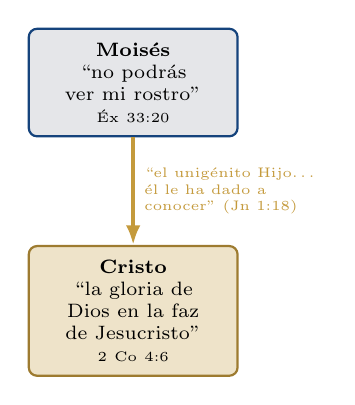
\begin{tikzpicture}[font=\scriptsize]
 \node[caja,text width=2.3cm,align=center,fill=gris!15] (m) at (0,1.6) {\textbf{Moisés}\\ ``no podrás ver mi rostro''\\ {\tiny Éx 33:20}};
 \node[caja,text width=2.3cm,align=center,fill=dorado!30,draw=dorado!80!black] (c) at (0,-1.3) {\textbf{Cristo}\\ ``la gloria de Dios en la faz de Jesucristo''\\ {\tiny 2 Co 4:6}};
 \draw[-{Latex[length=2.5mm]},dorado,line width=1.4pt] (m)--(c) node[midway,right,text width=2.2cm,font=\tiny]{``el unigénito Hijo\ldots{} él le ha dado a conocer'' (Jn 1:18)};
\end{tikzpicture}
\end{column}
\end{columns}
\end{frame}

% ------------------------------------------------------------------
\section{La palabra}

\begin{frame}{\emph{Kavod}: el peso de Dios}
\begin{columns}[c,onlytextwidth]
\begin{column}{0.56\textwidth}
\scriptsize\renewcommand{\arraystretch}{1.15}
\begin{tabular}{@{}>{\RaggedRight\arraybackslash}p{1.1cm}>{\RaggedRight\arraybackslash}p{2.3cm}>{\RaggedRight\arraybackslash}p{3.4cm}@{}}
\toprule
\textbf{Texto} & \textbf{Hebreo} & \textbf{Sentido concreto} \\ \midrule
Gn 13:2 & \heb{כָּבֵד מְאֹד} & Abram ``riquísimo'': pesado en bienes \\
Gn 31:1 & \heb{הַכָּבֹד הַזֶּה} & ``esta riqueza'': primer \emph{kavod} \\
Éx 4:10 & \heb{כְבַד־פֶּה} & ``tardo en el habla'': pesado de boca \\
Éx 7:14 & \heb{כָּבֵד לֵב} & corazón de Faraón ``endurecido'' \\
Éx 20:12 & \heb{כַּבֵּד} & ``honra'' a tu padre: dale peso \\
1 S 4:18 & \heb{וְכָבֵד} & Elí, ``viejo y pesado'' \\
Sal 16:9 & \heb{כְּבוֹדִי} & ``mi alma'': lo más valioso del ser \\
\bottomrule
\end{tabular}
\end{column}
\begin{column}{0.42\textwidth}\small
\begin{itemize}
\item Raíz \heb{כבד} \emph{k-b-d}: \destacar{ser pesado}.
\item Lo pesado es lo valioso: honrar es \destacar{dar peso}; despreciar es tener por liviano (\heb{קלל}).
\item ``Yo honraré (\heb{אֲכַבֵּד}) a los que me honran, y los que me desprecian serán tenidos en poco (\heb{יֵקָלּוּ})'' (1 S 2:30).
\end{itemize}
\end{column}
\end{columns}
\end{frame}

\begin{frame}{Seis sentidos de \emph{kavod}}
\centering
\begin{tikzpicture}[font=\scriptsize]
 \node[circle,draw=dorado,line width=1.6pt,fill=azul,text=papiro,minimum size=1.7cm,align=center] (k) at (0,0) {\heb{כָּבוֹד}\\ \emph{kavod}};
 \foreach \a/\t/\d in {90/{Peso, abundancia}/{Gn 31:1; Os 9:11},30/{Honra, reputación}/{Gn 45:13; Sal 8:5},330/{El yo, el alma}/{Gn 49:6; Sal 57:8},270/{Resplandor visible}/{Éx 16:10; 40:34},210/{Dios en plenitud}/{Éx 33:18; Is 6:3},150/{Gloria que se le da}/{Sal 29:1--2; 115:1}}{
  \node[caja,text width=2.3cm,align=center] (n\a) at (\a:2.65) {\textbf{\t}\\ {\tiny\color{gris}\d}};
  \draw[dorado,line width=1pt] (k)--(n\a);}
\end{tikzpicture}\par\smallskip
{\scriptsize Maimónides (\emph{Guía} I:64): el término es homónimo: luz creada (Éx 24:16), esencia de Dios (Éx 33:18), glorificación (Sal 29:9).}
\end{frame}

\begin{frame}{El espectro de ``gloria''}
\scriptsize\renewcommand{\arraystretch}{1.1}
\begin{columns}[t,onlytextwidth]
\begin{column}{0.50\textwidth}
\begin{tabular}{@{}>{\RaggedRight\arraybackslash}p{2.4cm}>{\RaggedRight\arraybackslash}p{3.3cm}@{}}
\toprule
\textbf{Hebreo / arameo} & \textbf{Sentido} \\ \midrule
\heb{כָּבוֹד} \emph{kavod} & peso, honra, gloria, resplandor \\
\heb{כָּבֵד}, \heb{נִכְבַּד} & honrar; ser glorificado \\
\heb{תִּפְאֶרֶת} \emph{tif'éret} & hermosura, ornamento \\
\heb{הוֹד} \emph{hod}, \heb{הָדָר} \emph{hadar} & majestad, esplendor \\
\heb{צְבִי} \emph{tsevi} & ornamento, gloria \\
\heb{הִתְהַלֵּל} \emph{hithalel} & gloriarse, alabarse \\
\heb{יְקָר} \emph{yeqar} (aram.) & honra, gloria \\
\bottomrule
\end{tabular}
\end{column}
\begin{column}{0.48\textwidth}
\begin{tabular}{@{}>{\RaggedRight\arraybackslash}p{2.5cm}>{\RaggedRight\arraybackslash}p{2.9cm}@{}}
\toprule
\textbf{Griego} & \textbf{Sentido} \\ \midrule
\grc{δόξα} \emph{doxa} & gloria (166 veces) \\
\grc{δοξάζω} \emph{doxazō} & glorificar (61) \\
\grc{συνδοξάζω} & glorificados con él \\
\grc{καυχάομαι} & gloriarse (38) \\
\grc{κενοδοξία} & vanagloria \\
\grc{μεγαλοπρεπής} & ``magnífica'' gloria \\
\bottomrule
\end{tabular}
\end{column}
\end{columns}\par\medskip
\small RVR1960: la familia de ``gloria'' \textbf{568 veces} en \textbf{516 versículos}. El sustantivo \emph{kavod}: \textbf{199 veces} en \textbf{188 versículos}; Salmos 51, Isaías 37, Ezequiel 18.\par
\precision{conteo propio (RVR1960 sin títulos; BHS por raíz; NA27 con Strong). Vine da 200 para \emph{kavod}. Verificar en e-Sword.}
\end{frame}

\begin{frame}{\emph{Doxa}: de la opinión al resplandor}
\centering
\begin{tikzpicture}[font=\scriptsize,node distance=0.75cm,
  b/.style={caja,text width=2.9cm,align=center},a/.style={-{Latex[length=2.6mm]},dorado,line width=1.4pt}]
 \node[b] (h) {\textbf{Hebreo}\\[2pt] \heb{כָּבוֹד} \emph{kavod}\\ peso $\rightarrow$ honra $\rightarrow$ gloria};
 \node[b,right=of h] (g) {\textbf{Septuaginta}\\[2pt] \grc{δόξα} \emph{doxa}\\ ``opinión'' $\rightarrow$ resplandor de Dios};
 \node[b,right=of g] (p) {\textbf{Juan y Pablo}\\[2pt] \grc{δόξα} en Cristo\\ Jn 1:14; 2 Co 4:6};
 \draw[a] (h)--(g); \draw[a] (g)--(p);
\end{tikzpicture}\par\medskip
\begin{columns}[t,onlytextwidth]
\begin{column}{0.48\textwidth}\small
\grc{δόξα} viene de \grc{δοκέω}, ``parecer, opinar''. Tu aplicación: glorificar a Dios es vivir de modo que se \destacar{ensanche la opinión} que otros tienen de Él.
\end{column}
\begin{column}{0.48\textwidth}\small
Pink (2020, pp. 6--7): la ``gloria esencial'' de Dios ``no puede ser aumentada''; lo que crece es ``su gloria manifiesta y su reconocimiento por parte de nosotros''.
\end{column}
\end{columns}
\end{frame}

\begin{frame}{El rostro ``glorificado''}
\begin{columns}[c,onlytextwidth]
\begin{column}{0.50\textwidth}
\begin{center}\heb{כִּי קָרַן עוֹר פָּנָיו}\end{center}
\scriptsize\renewcommand{\arraystretch}{1.2}
\begin{tabular}{@{}>{\RaggedRight\arraybackslash}p{1.6cm}>{\RaggedRight\arraybackslash}p{4.4cm}@{}}
\toprule
TM & ``la piel de su rostro \emph{resplandecía}'' (\heb{קָרַן}, de \heb{קֶרֶן}, ``rayo, cuerno'') \\
LXX & \grc{δεδόξασται ἡ ὄψις}: ``\emph{había sido glorificada}'' \\
Vulgata & \emph{cornuta}: ``con cuernos'' (el Moisés de Miguel Ángel) \\
RVR1960 & ``resplandecía'' \\
\bottomrule
\end{tabular}
\end{column}
\begin{column}{0.48\textwidth}\small
\begin{itemize}
\item Éx 34:29: Moisés baja del Sinaí con el rostro radiante.
\item La LXX usa el verbo \grc{δοξάζω}: prueba del paso de \emph{doxa} a ``resplandor''.
\item Ese verbo, en ese verso, es el que Pablo comenta en \destacar{2 Corintios 3}.
\end{itemize}
\end{column}
\end{columns}\par\smallskip
\precision{(textual) este estudio sigue la lectura ``emitir rayos'' (LXX, RVR1960).}
\end{frame}

% ------------------------------------------------------------------
\section{El Nombre}

\begin{frame}{El nombre glorioso}
\begin{center}\heb{לְיִרְאָה אֶת־הַשֵּׁם הַנִּכְבָּד וְהַנּוֹרָא הַזֶּה אֵת יְהוָה אֱלֹהֶיךָ}\end{center}
\begin{cita}Si no cuidares de poner por obra todas las palabras de esta ley que están escritas en este libro, temiendo este nombre glorioso y temible: \textsc{Señor tu Dios}\ldots\fuente{(Dt 28:58)}\end{cita}
\scriptsize\renewcommand{\arraystretch}{1.15}
\begin{tabular}{@{}>{\RaggedRight\arraybackslash}p{2.4cm}>{\RaggedRight\arraybackslash}p{9.2cm}@{}}
\heb{הַשֵּׁם} \emph{hashem} & ``el Nombre'' por excelencia: de aquí \emph{HaShem}, como el judaísmo llama a Dios. \\
\heb{הַנִּכְבָּד} \emph{hanijbad} & ``glorioso'': \emph{nifal} de \heb{כבד}, ``el que tiene peso''. \destacar{El Nombre mismo es \emph{kavod}.} \\
\heb{וְהַנּוֹרָא} \emph{vehanorá} & ``y temible'': el peso de Dios se reconoce temiéndolo y obedeciendo. \\
\end{tabular}
\end{frame}

\begin{frame}{Los títulos de la gloria}
\scriptsize\renewcommand{\arraystretch}{1.14}
\begin{tabular}{@{}>{\RaggedRight\arraybackslash}p{2.7cm}>{\RaggedRight\arraybackslash}p{3.0cm}>{\RaggedRight\arraybackslash}p{2.0cm}>{\RaggedRight\arraybackslash}p{3.8cm}@{}}
\toprule
\textbf{Nombre o título} & \textbf{Hebreo / griego} & \textbf{Texto} & \textbf{Qué revela} \\ \midrule
El nombre glorioso & \heb{הַשֵּׁם הַנִּכְבָּד} & Dt 28:58 & El Nombre tiene peso \\
El Rey de gloria & \heb{מֶלֶךְ הַכָּבוֹד} & Sal 24:7--10 & Entra como rey victorioso \\
El Dios de gloria & \heb{אֵל־הַכָּבוֹד} & Sal 29:3 & Su voz sacude la creación \\
Mi gloria & \heb{כְּבוֹדִי} & Sal 3:3 & Es la gloria del creyente \\
El Dios de la gloria & \grc{ὁ θεὸς τῆς δόξης} & Hch 7:2 & Se apareció a Abraham \\
El Señor de gloria & \grc{τὸν κύριον τῆς δόξης} & 1 Co 2:8; Stg 2:1 & El título del Sal 24, dado al crucificado \\
El Padre de gloria & \grc{ὁ πατὴρ τῆς δόξης} & Ef 1:17 & Da sabiduría y revelación \\
El resplandor de su gloria & \grc{ἀπαύγασμα τῆς δόξης} & He 1:3 & El Hijo irradia la gloria \\
\bottomrule
\end{tabular}\par\medskip
\precision{la gloria no tiene un nombre propio como \emph{El Shaddai}; se revela en títulos que unen el Nombre con \emph{kavod}. Principio judío: ``según mis obras soy llamado'' (\emph{Shemot Rabá} 3:6).}
\end{frame}

% ------------------------------------------------------------------
\section{Definición}

\begin{frame}{¿Qué es la gloria de Dios?}
\begin{tcolorbox}[enhanced,colback=papiro,colframe=azul,boxrule=1pt,arc=3pt,title={Definición},fonttitle=\bfseries\small,colbacktitle=azul,coltitle=papiro,fontupper=\small]
La \textbf{gloria de Dios} (\heb{כְּבוֹד יְהוָה}; \grc{δόξα τοῦ θεοῦ}) es el \destacar{peso infinito de todo lo que Dios es}: la plenitud de sus atributos en perfecta comunión. Es eterna (Jn 17:5). Se \emph{manifiesta} en la creación (Sal 19:1), en la nube y el fuego (Éx 40:34), en su Nombre (Éx 34:6--7) y, en plenitud, en el rostro de Jesucristo (2 Co 4:6; Col 2:9). Se \emph{reconoce} cuando sus criaturas le dan el peso que le corresponde (Sal 29:2; 1 Co 10:31).
\end{tcolorbox}
\small Tu material: ``Cuando Dios deja ver lo que Él es, lo que se manifiesta es su gloria. \destacar{La gloria de Dios engloba todo lo que Él es}''. Vine: \emph{doxa} es ``lo que él esencialmente es y hace, tal y como queda exhibido en cualquier forma en que se revele a sí mismo''.
\end{frame}

\begin{frame}{Tres dimensiones}
\centering
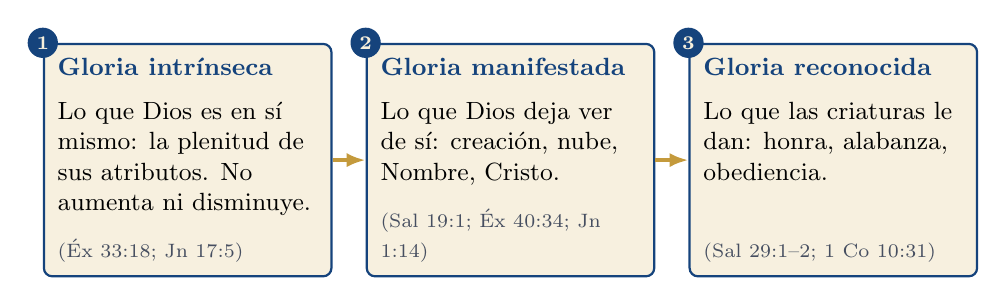
\begin{tikzpicture}
 \foreach \x/\n/\t/\d/\r in {0/1/{Gloria intrínseca}/{Lo que Dios es en sí mismo: la plenitud de sus atributos. No aumenta ni disminuye.}/{Éx 33:18; Jn 17:5},
   4.1/2/{Gloria manifestada}/{Lo que Dios deja ver de sí: creación, nube, Nombre, Cristo.}/{Sal 19:1; Éx 40:34; Jn 1:14},
   8.2/3/{Gloria reconocida}/{Lo que las criaturas le dan: honra, alabanza, obediencia.}/{Sal 29:1--2; 1 Co 10:31}}{
  \node[caja,anchor=north] (b\n) at (\x,0) {\parbox[t][2.6cm][t]{3.3cm}{\RaggedRight
    {\small\textbf{\textcolor{azul}{\t}}}\\[5pt]\small \d\par\vfill{\scriptsize\color{gris}(\r)}}};
  \node[circle,fill=azul,text=papiro,font=\scriptsize\bfseries,inner sep=1.6pt] at (b\n.north west) {\n};}
 \draw[-{Latex[length=2.4mm]},dorado,line width=1.4pt] (b1.east)--(b2.west);
 \draw[-{Latex[length=2.4mm]},dorado,line width=1.4pt] (b2.east)--(b3.west);
\end{tikzpicture}\par\medskip
\small\RaggedRight La primera no depende de nosotros; la segunda es iniciativa de Dios; la tercera es \destacar{nuestra respuesta}. ``Dad a \SENOR{} la gloria'' no le añade nada: reconoce el peso que ya tiene.
\end{frame}

\begin{frame}{Convergencia: por qué todos}
\begin{columns}[t,onlytextwidth]
\begin{column}{0.32\textwidth}
\begin{block}{1. Nunca un atributo solo}\scriptsize Éx 34:6--7: la gloria es el Nombre con sus atributos. Sal 115:1: ``por tu misericordia, por tu verdad''. Ro 11:33--36: sabiduría, ciencia, juicios $\rightarrow$ ``a él sea la gloria''.\end{block}
\end{column}
\begin{column}{0.32\textwidth}
\begin{block}{2. No se estorban}\scriptsize ``La misericordia y la verdad se encontraron; la justicia y la paz se besaron'' (Sal 85:10). Charnock en Pink: su nombre ``significa todos sus atributos en conjunto'' (Pink, 2020, p. 42).\end{block}
\end{column}
\begin{column}{0.32\textwidth}
\begin{block}{3. Tienen un lugar}\scriptsize ``Agradó al Padre que en él habitase toda plenitud'' (Col 1:19); ``en él habita corporalmente toda la plenitud de la Deidad'' (Col 2:9).\end{block}
\end{column}
\end{columns}\par\medskip
\precision{``comunión de todos los atributos'' es la tesis de esta obra; la teología clásica dice ``manifestación de las perfecciones de Dios'' (Berkhof, 1938; Charnock, 1682/1996).}
\end{frame}

% ------------------------------------------------------------------
\section{La Torá}

\begin{frame}{La Torá narra la gloria}
\scriptsize\renewcommand{\arraystretch}{1.08}
\begin{tabular}{@{}>{\RaggedRight\arraybackslash}p{1.9cm}>{\RaggedRight\arraybackslash}p{2.4cm}>{\RaggedRight\arraybackslash}p{3.6cm}>{\RaggedRight\arraybackslash}p{3.7cm}@{}}
\toprule
\textbf{Texto} & \textbf{Lugar} & \textbf{Cómo aparece} & \textbf{Ocasión y efecto} \\ \midrule
Éx 14:4, 17--18 & Mar Rojo & ``seré glorificado en Faraón'' & Juicio; ``sabrán que yo soy \SENOR'' \\
Éx 16:7, 10 & Desierto de Sin & ``apareció en la nube'' & Murmuración; maná \\
Éx 24:15--18 & Sinaí & ``reposó''; ``fuego abrasador'' & Pacto; Moisés sube 40 días \\
Éx 33:9--11 & Tienda de reunión & la columna ``descendía'' & Dios habla; el pueblo adora \\
Éx 33:18--34:8 & Peña & ``todo mi bien''; el Nombre & Intercesión tras el becerro \\
Éx 34:29--35 & Bajada & el rostro resplandece & Temor; el velo \\
Éx 40:34--38 & Tabernáculo & ``llenó el tabernáculo'' & Moisés no puede entrar \\
Lv 9:23--10:3 & Altar & fuego; ``seré glorificado'' & Culto; Nadab y Abiú \\
Nm 9:15--23 & Campamento & nube de día, fuego de noche & Parten y acampan ``al mandato'' \\
Nm 14:10, 21 & Cades & ``mi gloria llena toda la tierra'' & Perdón y juicio \\
Dt 28:58 & Moab & ``nombre glorioso y temible'' & Temer y obedecer \\
\bottomrule
\end{tabular}
\end{frame}

\begin{frame}{Glorificado en Faraón}
\begin{columns}[c,onlytextwidth]
\begin{column}{0.52\textwidth}
\begin{center}\heb{וְאִכָּבְדָה בְּפַרְעֹה}\end{center}
\begin{cita}Y yo endureceré el corazón de Faraón para que los siga; y seré glorificado en Faraón y en todo su ejército, y sabrán los egipcios que yo soy \SENOR.\fuente{(Éx 14:4)}\end{cita}
\end{column}
\begin{column}{0.46\textwidth}\small
\begin{itemize}
\item El corazón de Faraón estaba \heb{כָּבֵד}, ``\destacar{pesado}'' (Éx 7:14; 8:15, 32; 9:7, 34).
\item Dios dice \heb{וְאִכָּבְדָה}: ``\destacar{me haré pesado}'', ``seré glorificado''.
\item Salvación para Israel, juicio para Egipto; en ambos, \destacar{conocimiento}.
\item Al otro lado: ``magnífico en santidad'' (\heb{נֶאְדָּר בַּקֹּדֶשׁ}, Éx 15:11).
\end{itemize}
\end{column}
\end{columns}\par\smallskip
\precision{el juego corazón ``pesado'' / Dios ``glorificado'' es observación de la exégesis moderna; en 14:4 ``endurecer'' es otra raíz (\heb{חזק}).}
\end{frame}

\begin{frame}{Sinaí: la gloria que reposa}
\begin{center}\heb{וַיִּשְׁכֹּן כְּבוֹד־יְהוָה עַל־הַר סִינַי}\end{center}
\begin{cita}Entonces Moisés subió al monte, y una nube cubrió el monte. Y la gloria de \SENOR{} reposó sobre el monte Sinaí, y la nube lo cubrió por seis días; y al séptimo día llamó a Moisés de en medio de la nube. Y la apariencia de la gloria de \SENOR{} era como un fuego abrasador en la cumbre del monte, a los ojos de los hijos de Israel.\fuente{(Éx 24:15--17)}\end{cita}
\scriptsize \heb{וַיִּשְׁכֹּן} \emph{vayishkón}, ``reposó, habitó'': de \heb{שׁכן} vienen \heb{מִשְׁכָּן} (\emph{mishkán}, tabernáculo) y \heb{שְׁכִינָה} (\emph{Shejiná}). ``Seis días'' y ``el séptimo'': la gloria reposa al ritmo de la creación. ``Fuego que devora'' (\heb{כְּאֵשׁ אֹכֶלֶת}; cf. Dt 4:24).
\end{frame}


\begin{frame}{``Habitaré en medio de ellos''}
\begin{columns}[c,onlytextwidth]
\begin{column}{0.50\textwidth}
\begin{center}\heb{וְעָשׂוּ לִי מִקְדָּשׁ וְשָׁכַנְתִּי בְּתוֹכָם}\end{center}
\begin{cita}Y harán un santuario para mí, y habitaré en medio de ellos.\fuente{(Éx 25:8)}\end{cita}
\begin{cita}Allí me reuniré con los hijos de Israel; y el lugar será santificado con mi gloria\ldots{} Y habitaré entre los hijos de Israel, y seré su Dios.\fuente{(Éx 29:43, 45)}\end{cita}
\end{column}
\begin{column}{0.48\textwidth}\small
\begin{itemize}
\item Dios no pide una casa para encerrarse, sino para estar \destacar{en medio} del pueblo.
\item El centro: el arca y el propiciatorio: ``de allí\ldots{} hablaré contigo'' (Éx 25:22).
\item Las vestiduras: ``para honra y hermosura'' (\heb{לְכָבוֹד וּלְתִפְאָרֶת}, Éx 28:2).
\end{itemize}
\precision{Ónkelos: ``haré reposar mi Shejiná entre ellos''; LXX: ``seré visto entre vosotros''. Ambas evitan que Dios ``quepa'' en un lugar.}
\end{column}
\end{columns}
\end{frame}

\begin{frame}{La columna que desciende}
\begin{columns}[c,onlytextwidth]
\begin{column}{0.52\textwidth}
\begin{center}\heb{יֵרֵד עַמּוּד הֶעָנָן וְעָמַד פֶּתַח הָאֹהֶל}\end{center}
\begin{cita}Cuando Moisés entraba en el tabernáculo, la columna de nube descendía y se ponía a la puerta del tabernáculo, y \SENOR{} hablaba con Moisés. Y viendo todo el pueblo la columna de nube que estaba a la puerta del tabernáculo, se levantaba cada uno a la puerta de su tienda y adoraba.\fuente{(Éx 33:9--10)}\end{cita}
\end{column}
\begin{column}{0.46\textwidth}
\centering
\begin{tikzpicture}[font=\scriptsize]
 \foreach \y/\n/\t/\r in {2.1/1/{Desciende}/{\heb{יָרַד} Éx 33:9; Nm 12:5},0.7/2/{Se detiene a la puerta}/{\heb{עָמַד} Éx 33:9},-0.7/3/{Habla}/{Éx 33:9, 11; Nm 7:89},-2.1/4/{El pueblo adora}/{Éx 33:10}}{
  \node[caja,text width=3.6cm,align=left] (s\n) at (0,\y) {\textbf{\textcolor{azul}{\t}}\\ {\tiny\color{gris}\r}};}
 \foreach \i/\j in {1/2,2/3,3/4}{\draw[-{Latex[length=2mm]},dorado,line width=1.2pt] (s\i)--(s\j);}
\end{tikzpicture}
\end{column}
\end{columns}\par\smallskip
\scriptsize La gloria no se queda en la cumbre: \destacar{baja al nivel del campamento}. ``\SENOR{} descendió en la columna de la nube, y se puso a la puerta del tabernáculo'' (Nm 12:5).
\end{frame}

\begin{frame}{La gloria llena el tabernáculo}
\fotolado{panel_exodo40.jpg}{Elaboración propia: Éx 40:34 en texto hebreo consonántico (BHS).}
\begin{columns}[c,onlytextwidth]
\begin{column}{0.57\textwidth}
\begin{cita}Entonces una nube cubrió el tabernáculo de reunión, y la gloria de \SENOR{} llenó el tabernáculo. Y no podía Moisés entrar en el tabernáculo de reunión, porque la nube estaba sobre él, y la gloria de \SENOR{} lo llenaba.\fuente{(Éx 40:34--35)}\end{cita}
\scriptsize
\heb{מָלֵא} \emph{malé}, ``llenó'': el verbo de Is 6:3. \heb{שָׁכַן עָלָיו הֶעָנָן}: la nube ``habitaba'' sobre él; LXX \grc{ἐπεσκίαζεν}, ``cubría con su sombra'', el verbo de Lc 1:35 y 9:34.\par\smallskip
Éxodo empieza con ladrillos para Faraón y termina con \destacar{la gloria en medio de Israel}.
\end{column}
\begin{column}{0.41\textwidth}\end{column}
\end{columns}
\end{frame}

\begin{frame}{La morada}
\centering
\begin{tikzpicture}[font=\scriptsize,scale=0.86,transform shape]
 \draw[azul,line width=0.9pt,fill=papiro] (0,0) rectangle (12,4.6);
 \node[anchor=north west,text=gris] at (0.1,4.55) {Atrio (Éx 27:9--18)};
 \draw[azul,fill=dorado!25] (1.6,1.7) rectangle (2.8,2.9); \node at (2.2,2.3) {Altar};
 \node[text=gris,font=\tiny] at (2.2,1.35) {Lv 9:24: fuego};
 \draw[azul,fill=celeste!30] (4.0,2.3) circle (0.4); \node[font=\tiny] at (4.0,1.65) {Fuente};
 \draw[azul,line width=1pt,fill=azul!8] (5.0,1.2) rectangle (11.4,3.4);
 \draw[azul,line width=0.8pt] (8.8,1.2)--(8.8,3.4);
 \node[font=\scriptsize\bfseries] at (6.9,2.85) {Lugar santo};
 \node[align=center,font=\tiny] at (6.9,2.05) {candelero, mesa,\\ altar del incienso};
 \node[align=center,text width=2.3cm,font=\scriptsize\bfseries] at (10.1,2.85) {Lugar santísimo};
 \draw[dorado!80!black,fill=dorado!60] (9.6,1.55) rectangle (10.6,2.05);
 \node[font=\tiny] at (10.1,0.95) {arca y propiciatorio};
 \foreach \x/\y/\r in {9.4/4.9/0.5,10.1/5.15/0.6,10.8/4.9/0.5,9.8/4.7/0.45,10.5/4.7/0.45}{\fill[gris!25] (\x,\y) circle (\r);}
 \node[text=azuloscuro] at (10.1,4.95) {\textbf{nube}};
 \draw[-{Latex[length=2.4mm]},dorado,line width=1.4pt] (10.1,4.25)--(10.1,3.45);
 \node[anchor=west,text width=4cm,align=left] at (12.3,4.3) {\textbf{\textcolor{azul}{La gloria llena la morada}}\\ Éx 40:34--35; Lv 16:2:\\ ``apareceré en la nube sobre el propiciatorio''};
 \node[anchor=west,text width=4cm,align=left] at (12.3,1.8) {\heb{מִשְׁכָּן} \emph{mishkán}, ``morada''\\ \heb{שָׁכַן} \emph{shakhán}, ``habitar''\\ $\rightarrow$ \grc{ἐσκήνωσεν} (Jn 1:14)};
\end{tikzpicture}\par
{\fontsize{5}{6}\selectfont\color{gris}\textit{Nota.} Elaboración propia: esquema simplificado del tabernáculo (Éx 25--27; 40), sin escala.\par}
\begin{columns}[t,onlytextwidth]
\begin{column}{0.32\textwidth}\scriptsize\textbf{\textcolor{azul}{Llena y excluye}}: ni Moisés puede entrar (Éx 40:35; 1 R 8:11).\end{column}
\begin{column}{0.32\textwidth}\scriptsize\textbf{\textcolor{azul}{Guía}}: ``al mandato de \SENOR{} partían, y al mandato de \SENOR{} acampaban'' (Nm 9:18).\end{column}
\begin{column}{0.32\textwidth}\scriptsize\textbf{\textcolor{azul}{Habita en una tienda}}: ``habitó (\grc{ἐσκήνωσεν}) entre nosotros, y vimos su gloria'' (Jn 1:14).\end{column}
\end{columns}
\end{frame}

\begin{frame}{Los verbos de la gloria}
\scriptsize\renewcommand{\arraystretch}{1.16}
\begin{tabular}{@{}>{\RaggedRight\arraybackslash}p{3.1cm}>{\RaggedRight\arraybackslash}p{4.0cm}>{\RaggedRight\arraybackslash}p{4.5cm}@{}}
\toprule
\textbf{Verbo} & \textbf{Textos} & \textbf{Qué hace la gloria} \\ \midrule
\heb{יָרַד} \emph{yarad}, descender & Éx 19:20; 33:9; 34:5; Nm 12:5; 2 Cr 7:1 & Baja al monte, a la puerta, al altar \\
\heb{שָׁכַן} \emph{shakhán}, habitar & Éx 24:16; 25:8; 40:35; Nm 9:17 & Se queda: \emph{mishkán}, \emph{Shejiná} \\
\heb{כָּסָה} \emph{kasá}, cubrir & Éx 24:15; 40:34; Nm 9:15 & Revela que Dios está, sin mostrarlo \\
\heb{מָלֵא} \emph{malé}, llenar & Éx 40:34; 1 R 8:11; 2 Cr 5:14; Is 6:3 & Ocupa todo; nadie puede entrar \\
\heb{נִרְאָה} \emph{nir'á}, aparecer & Éx 16:10; Lv 9:23; Nm 14:10 & Visible en la crisis y en el culto \\
\heb{דִּבֶּר} \emph{dibbér}, hablar & Éx 25:22; 33:9; Nm 7:89 & De entre los querubines sale la voz \\
\heb{עָלָה} \emph{alá}, alzarse & Éx 40:36; Nm 9:17; Ez 11:23 & Se levanta para guiar\ldots{} o para irse \\
\bottomrule
\end{tabular}\par\medskip
\precision{selección propia de verbos, tomados del hebreo de cada pasaje.}
\end{frame}

\begin{frame}{Fuego en el altar}
\begin{columns}[c,onlytextwidth]
\begin{column}{0.50\textwidth}
\begin{center}\heb{בִּקְרֹבַי אֶקָּדֵשׁ וְעַל־פְּנֵי כָל־הָעָם אֶכָּבֵד}\end{center}
\begin{cita}Esto es lo que habló \SENOR, diciendo: En los que a mí se acercan me santificaré, y en presencia de todo el pueblo seré glorificado. Y Aarón calló.\fuente{(Lv 10:3)}\end{cita}
\end{column}
\begin{column}{0.48\textwidth}\small
\begin{itemize}
\item Lv 9:23--24: ``la gloria de \SENOR{} se apareció a todo el pueblo'' y el fuego consume el holocausto.
\item Lv 10:1--2: el mismo fuego consume a Nadab y Abiú.
\item Paralelismo: ``me santificaré'' $\parallel$ ``seré glorificado'': la gloria es la de un \destacar{Dios santo}.
\item El silencio de Aarón: la reacción ante el peso de Dios.
\end{itemize}
\end{column}
\end{columns}
\end{frame}

\begin{frame}{``Mi gloria llena toda la tierra''}
\begin{center}\heb{וְאוּלָם חַי־אָנִי וְיִמָּלֵא כְבוֹד־יְהוָה אֶת־כָּל־הָאָרֶץ}\end{center}
\begin{cita}Entonces \SENOR{} dijo: Yo lo he perdonado conforme a tu dicho. Mas tan ciertamente como vivo yo, y mi gloria llena toda la tierra, todos los que vieron mi gloria y mis señales que he hecho en Egipto y en el desierto, y me han tentado ya diez veces, y no han oído mi voz, no verán la tierra de la cual juré a sus padres.\fuente{(Nm 14:20--23)}\end{cita}
\small Perdón y juicio juntos, como Éx 34:7. La gloria de una tienda llenará \destacar{toda la tierra} (Sal 72:19; Is 6:3; Hab 2:14). El problema de esa generación: haber \destacar{visto} la gloria y no \destacar{oído} su voz.
\end{frame}

% ------------------------------------------------------------------
\section{En Israel}

\begin{frame}{Elí y sus hijos}
\begin{columns}[c,onlytextwidth]
\begin{column}{0.54\textwidth}
\begin{center}\heb{כִּי־מְכַבְּדַי אֲכַבֵּד וּבֹזַי יֵקָלּוּ}\end{center}
\begin{cita}¿Por qué\ldots{} has honrado a tus hijos más que a mí, engordándoos de lo principal de todas las ofrendas de mi pueblo Israel?\ldots{} porque yo honraré a los que me honran, y los que me desprecian serán tenidos en poco.\fuente{(1 S 2:29--30)}\end{cita}
\end{column}
\begin{column}{0.44\textwidth}\small
\begin{itemize}
\item Elí ``honró'' (\heb{וַתְּכַבֵּד}, ``diste peso'') a sus hijos más que a Dios.
\item Israel lleva el arca a la batalla ``para que\ldots{} nos salve'' (1 S 4:3): \destacar{la presencia sin la obediencia}.
\item ``Fue hecha muy grande mortandad\ldots{} Y el arca de Dios fue tomada'' (1 S 4:10--11).
\end{itemize}
\end{column}
\end{columns}
\end{frame}

\begin{frame}{``Viejo y pesado''}
\begin{columns}[c,onlytextwidth]
\begin{column}{0.52\textwidth}
\begin{center}\heb{כִּי־זָקֵן הָאִישׁ וְכָבֵד}\end{center}
\begin{cita}Y aconteció que cuando él hizo mención del arca de Dios, Elí cayó hacia atrás de la silla al lado de la puerta, y se desnucó y murió; porque era hombre viejo y pesado. Y había juzgado a Israel cuarenta años.\fuente{(1 S 4:18)}\end{cita}
\end{column}
\begin{column}{0.46\textwidth}
\centering
\begin{tikzpicture}[font=\scriptsize]
 \node[caja,text width=3.6cm,align=center] (a) at (0,1.8) {\heb{כִּבֵּד} \emph{kibbed}, ``honrar''\\ honró a sus hijos (2:29)};
 \node[caja,text width=3.6cm,align=center] (b) at (0,0.3) {\heb{כָּבֵד} \emph{kaved}, ``pesado''\\ muere aplastado (4:18)};
 \node[caja,text width=3.6cm,align=center,fill=gris!18] (c) at (0,-1.2) {\heb{אִי־כָבוֹד} \emph{I-javod}\\ ``¿dónde está la gloria?'' (4:21)};
 \draw[-{Latex[length=2mm]},dorado,line width=1.2pt] (a)--(b); \draw[-{Latex[length=2mm]},dorado,line width=1.2pt] (b)--(c);
\end{tikzpicture}\par\smallskip
\precision{el juego de la raíz lo señalan comentaristas del hebreo (Alter, 1999); la lectura ``pesado de sí, liviano para Dios'' es aplicación propia.}
\end{column}
\end{columns}
\end{frame}

\begin{frame}{Icabod}
\fotolado{panel_1samuel4.jpg}{Elaboración propia: 1 S 4:21 en texto hebreo consonántico (BHS).}
\begin{columns}[c,onlytextwidth]
\begin{column}{0.57\textwidth}
\begin{cita}Y llamó al niño Icabod, diciendo: ¡Traspasada es la gloria de Israel! por haber sido tomada el arca de Dios, y por la muerte de su suegro y de su marido. Dijo, pues: Traspasada es la gloria de Israel; porque ha sido tomada el arca de Dios.\fuente{(1 S 4:21--22)}\end{cita}
\scriptsize
\heb{אִי־כָבוֹד}: \heb{אִי} interrogativa (``¿dónde está la gloria?'') o negativa (``sin gloria''): la gloria no está (BDB; HALOT).\par
\heb{גָּלָה} \emph{galá}, ``traspasada'': el verbo técnico del \destacar{exilio}. ``La gloria se fue al destierro''.\par
La madre entiende lo que se perdió: no el ejército, sino \destacar{la presencia de Dios}.
\end{column}
\begin{column}{0.41\textwidth}\end{column}
\end{columns}
\end{frame}

\begin{frame}{Del arca perdida a David}
\centering
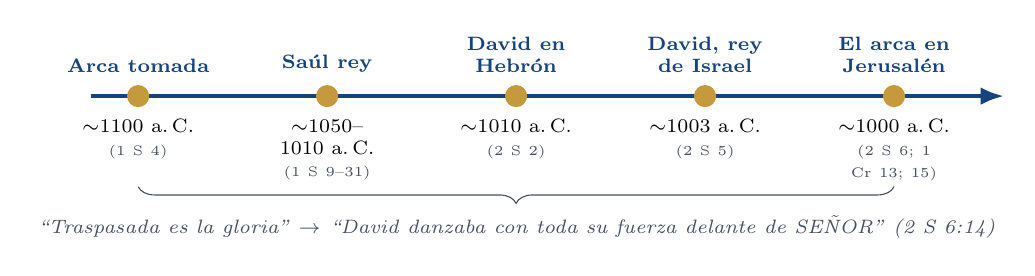
\begin{tikzpicture}[font=\scriptsize]
 \draw[line width=1.6pt,azul,-{Latex[length=3mm]}] (0,0)--(11.6,0);
 \foreach \x/\a/\t/\r in {0.6/{$\sim$1100}/{Arca tomada}/{1 S 4},3.0/{$\sim$1050--1010}/{Saúl rey}/{1 S 9--31},5.4/{$\sim$1010}/{David en Hebrón}/{2 S 2},7.8/{$\sim$1003}/{David, rey de Israel}/{2 S 5},10.2/{$\sim$1000}/{El arca en Jerusalén}/{2 S 6; 1 Cr 13; 15}}{
   \fill[dorado] (\x,0) circle (4pt);
   \node[above=5pt,font=\scriptsize\bfseries,text=azul,align=center,text width=2.1cm] at (\x,0) {\t};
   \node[below=5pt,align=center,text width=2.1cm] at (\x,0) {\a{} a.\,C.\\{\tiny\color{gris}(\r)}};}
 \draw[decorate,decoration={brace,amplitude=6pt,mirror},gris] (0.6,-1.15)--(10.2,-1.15) node[midway,below=7pt,text=gris,font=\scriptsize\itshape] {``Traspasada es la gloria'' $\rightarrow$ ``David danzaba con toda su fuerza delante de \SENOR'' (2 S 6:14)};
\end{tikzpicture}\par\medskip
\begin{columns}[t,onlytextwidth]
\begin{column}{0.48\textwidth}\scriptsize Uza muere al tocar el arca (2 S 6:6--7): \destacar{la gloria no se maneja}, se recibe en los términos de Dios.\end{column}
\begin{column}{0.48\textwidth}\scriptsize David se hace liviano ante Dios: ``me haré más vil\ldots{} pero seré honrado'' (\heb{אִכָּבֵדָה}, 2 S 6:22). Es 1 S 2:30 cumplido.\end{column}
\end{columns}\par\smallskip
\precision{fechas aproximadas (cronología tradicional; otros sitúan Afec hacia 1050 a.\,C.). La tabla es la de tu material.}
\end{frame}

\begin{frame}{La gloria baja cuando se canta}
\begin{columns}[c,onlytextwidth]
\begin{column}{0.56\textwidth}
\begin{center}\heb{כִּי טוֹב כִּי לְעוֹלָם חַסְדּוֹ וְהַבַּיִת מָלֵא עָנָן}\end{center}
\begin{cita}\ldots{} y alababan a \SENOR, diciendo: Porque él es bueno, porque su misericordia es para siempre; entonces la casa se llenó de una nube, la casa de \SENOR. Y no podían los sacerdotes estar allí para ministrar, por causa de la nube; porque la gloria de \SENOR{} había llenado la casa de Dios.\fuente{(2 Cr 5:13--14)}\end{cita}
\end{column}
\begin{column}{0.42\textwidth}\small
\begin{itemize}
\item La nube llena el templo cuando Israel canta \destacar{dos atributos}: bondad (\heb{טוֹב}) y misericordia eterna (\heb{חַסְדּוֹ}).
\item 2 Cr 7:1--3: ``descendió fuego de los cielos\ldots{} y la gloria de \SENOR{} llenó la casa''; el pueblo canta lo mismo.
\item \destacar{La tesis hecha liturgia.}
\end{itemize}
\end{column}
\end{columns}\par\smallskip
\precision{la secuencia canto $\rightarrow$ nube es propia de Crónicas; 1 R 8:10--11 no menciona el canto.}
\end{frame}

\begin{frame}{El viaje de la gloria}
\centering
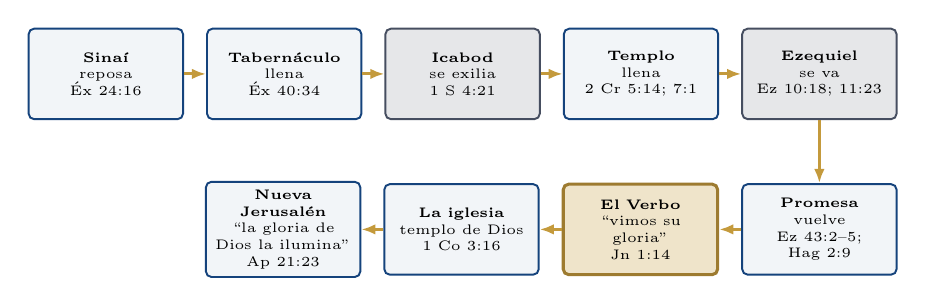
\begin{tikzpicture}[font=\tiny,node distance=0.28cm,
  e/.style={draw=azul,line width=0.7pt,fill=azul!6,fill opacity=0.9,text opacity=1,rounded corners=2pt,text width=1.75cm,align=center,inner sep=3pt,minimum height=1.15cm},
  f/.style={e,draw=gris,fill=gris!15},
  a/.style={-{Latex[length=1.8mm]},dorado,line width=1.1pt}]
 \node[e] (1) {\textbf{Sinaí}\\ reposa\\ Éx 24:16};
 \node[e,right=of 1] (2) {\textbf{Tabernáculo}\\ llena\\ Éx 40:34};
 \node[f,right=of 2] (3) {\textbf{Icabod}\\ se exilia\\ 1 S 4:21};
 \node[e,right=of 3] (4) {\textbf{Templo}\\ llena\\ 2 Cr 5:14; 7:1};
 \node[f,right=of 4] (5) {\textbf{Ezequiel}\\ se va\\ Ez 10:18; 11:23};
 \node[e,below=0.8cm of 5] (6) {\textbf{Promesa}\\ vuelve\\ Ez 43:2--5; Hag 2:9};
 \node[e,left=of 6,fill=dorado!30,draw=dorado!80!black,line width=1.1pt] (7) {\textbf{El Verbo}\\ ``vimos su gloria''\\ Jn 1:14};
 \node[e,left=of 7] (8) {\textbf{La iglesia}\\ templo de Dios\\ 1 Co 3:16};
 \node[e,left=of 8] (9) {\textbf{Nueva Jerusalén}\\ ``la gloria de Dios la ilumina''\\ Ap 21:23};
 \foreach \i/\j in {1/2,2/3,3/4,4/5,5/6,6/7,7/8,8/9}{\draw[a] (\i)--(\j);}
\end{tikzpicture}\par
{\fontsize{5}{6}\selectfont\color{gris}\textit{Nota.} Elaboración propia. En gris, los momentos en que la gloria se aleja.\par}\medskip
\begin{columns}[t,onlytextwidth]
\begin{column}{0.32\textwidth}\scriptsize\textbf{\textcolor{azul}{Santa}}: ``Santo, santo, santo\ldots{} toda la tierra está llena de su gloria'' (Is 6:3); ``vio su gloria'' (Jn 12:41).\end{column}
\begin{column}{0.32\textwidth}\scriptsize\textbf{\textcolor{azul}{Exclusiva}}: ``a otro no daré mi gloria, ni mi alabanza a esculturas'' (Is 42:8); LXX \grc{τὰς ἀρετάς μου}.\end{column}
\begin{column}{0.32\textwidth}\scriptsize\textbf{\textcolor{azul}{Universal}}: ``toda carne juntamente la verá'' (Is 40:5); ``Levántate, resplandece'' (Is 60:1).\end{column}
\end{columns}
\end{frame}

% ------------------------------------------------------------------
\section{Los Salmos}

\begin{frame}{Los cielos cuentan}
\fotolado{panel_salmo19.jpg}{Elaboración propia: Sal 19:1 [19:2] en texto hebreo consonántico (BHS).}
\begin{columns}[c,onlytextwidth]
\begin{column}{0.57\textwidth}
\begin{cita}Los cielos cuentan la gloria de Dios,\\ Y el firmamento anuncia la obra de sus manos.\\ Un día emite palabra a otro día,\\ Y una noche a otra noche declara sabiduría.\fuente{(Sal 19:1--2 [19:2--3])}\end{cita}
\scriptsize
\heb{מְסַפְּרִים} \emph{mesaprim}: ``cuentan'', narran sin pausa. \heb{כְּבוֹד־אֵל}: ``la gloria de \emph{El}''.\par\smallskip
Dos mitades: \destacar{la creación} (vv. 1--6, \emph{El}) y \destacar{la Torá} (vv. 7--14, \SENOR{} siete veces). La creación cuenta la gloria, pero no ``convierte el alma'' (v. 7).
\end{column}
\begin{column}{0.41\textwidth}\end{column}
\end{columns}
\end{frame}

\begin{frame}{Coronado de gloria}
\begin{columns}[c,onlytextwidth]
\begin{column}{0.50\textwidth}
\begin{center}\heb{וְכָבוֹד וְהָדָר תְּעַטְּרֵהוּ}\end{center}
\begin{cita}Cuando veo tus cielos, obra de tus dedos,\\ La luna y las estrellas que tú formaste,\\ Digo: ¿Qué es el hombre, para que tengas de él memoria,\\ Y el hijo del hombre, para que lo visites?\\ Le has hecho poco menor que los ángeles,\\ Y lo coronaste de gloria y de honra.\fuente{(Sal 8:3--5 [8:4--6])}\end{cita}
\end{column}
\begin{column}{0.48\textwidth}\small
\begin{itemize}
\item Marco: ``¡Cuán glorioso (\heb{אַדִּיר}) es tu nombre en toda la tierra!'' (vv. 1, 9).
\item El ser humano, \destacar{coronado de \emph{kavod}}: gloria recibida, reflejo.
\item He 2:9: ``vemos\ldots{} a Jesús, coronado de gloria y de honra, a causa del padecimiento de la muerte''.
\end{itemize}
\precision{\heb{מֵאֱלֹהִים}: el hebreo dice \emph{Elohim}; LXX \grc{παρ᾿ ἀγγέλους}, seguida por He 2:7 y la RVR1960.}
\end{column}
\end{columns}
\end{frame}

\begin{frame}{El Rey de gloria}
\begin{columns}[c,onlytextwidth]
\begin{column}{0.48\textwidth}
\begin{cita}Alzad, oh puertas, vuestras cabezas,\\ Y alzaos vosotras, puertas eternas,\\ Y entrará el Rey de gloria.\\ ¿Quién es este Rey de gloria?\\ \SENOR{} el fuerte y valiente,\\ \SENOR{} el poderoso en batalla\ldots\\ ¿Quién es este Rey de gloria?\\ \SENOR{} de los ejércitos,\\ El es el Rey de la gloria.\fuente{(Sal 24:7--10)}\end{cita}
\end{column}
\begin{column}{0.50\textwidth}\small
\begin{center}\heb{מִי הוּא זֶה מֶלֶךְ הַכָּבוֹד}\end{center}
\begin{itemize}
\item Liturgia de pregunta y respuesta; ``Rey de gloria'' \destacar{cinco veces}.
\item Las respuestas son atributos: fuerte, valiente, poderoso, de los ejércitos.
\item LXX \grc{ὁ βασιλεὺς τῆς δόξης} $\rightarrow$ Pablo: ``\destacar{el Señor de gloria}'' crucificado (1 Co 2:8).
\end{itemize}
\precision{la entrada del arca (2 S 6) o al templo (\emph{Shabat} 30a, Salomón) es lectura del contexto litúrgico.}
\end{column}
\end{columns}
\end{frame}

\begin{frame}{La morada de tu gloria}
\begin{columns}[t,onlytextwidth]
\begin{column}{0.48\textwidth}
\begin{center}\heb{וּמְקוֹם מִשְׁכַּן כְּבוֹדֶךָ}\end{center}
\begin{cita}\SENOR, la habitación de tu casa he amado,\\ Y el lugar de la morada de tu gloria.\fuente{(Sal 26:8)}\end{cita}
\scriptsize ``El lugar del \emph{mishkán} de tu \emph{kavod}'': las dos palabras de Éx 40:34.
\end{column}
\begin{column}{0.50\textwidth}
\begin{center}\heb{לִרְאוֹת עֻזְּךָ וּכְבוֹדֶךָ}\end{center}
\begin{cita}Para ver tu poder y tu gloria,\\ Así como te he mirado en el santuario.\\ Porque mejor es tu misericordia que la vida;\\ Mis labios te alabarán.\fuente{(Sal 63:2--3 [63:3--4])}\end{cita}
\scriptsize En el desierto de Judá (título): quien vio la gloria \destacar{tiene sed} de ella. Otra vez con atributos: poder y misericordia.
\end{column}
\end{columns}
\end{frame}

\begin{frame}{Dad a \SENOR{} la gloria}
\begin{columns}[c,onlytextwidth]
\begin{column}{0.50\textwidth}
\begin{center}\heb{הָבוּ לַיהוָה כְּבוֹד שְׁמוֹ}\end{center}
\begin{cita}Dad a \SENOR{} la gloria debida a su nombre;\\ Adorad a \SENOR{} en la hermosura de la santidad.\\ Voz de \SENOR{} sobre las aguas;\\ Truena el Dios de gloria\ldots\fuente{(Sal 29:2--3)}\end{cita}
\scriptsize ``Voz de \SENOR'' siete veces; \emph{kavod} cuatro. En el templo, \heb{כֻּלּוֹ אֹמֵר כָּבוֹד}: ``todo él dice: ¡Gloria!'' (v. 9).
\end{column}
\begin{column}{0.48\textwidth}
\begin{center}\heb{עַל כָּל־הָאָרֶץ כְּבוֹדֶךָ}\end{center}
\begin{cita}Exaltado seas sobre los cielos, oh Dios;\\ Sobre toda la tierra sea tu gloria.\fuente{(Sal 57:5, 11 [57:6, 12])}\end{cita}
\scriptsize Estribillo que separa la súplica en la cueva del canto del liberado. Sal 96:3: ``Proclamad entre las naciones su gloria''.
\end{column}
\end{columns}
\end{frame}

\begin{frame}{Gloria y atributos}
\begin{columns}[c,onlytextwidth]
\begin{column}{0.50\textwidth}
\begin{center}\heb{חֶסֶד־וֶאֱמֶת נִפְגָּשׁוּ צֶדֶק וְשָׁלוֹם נָשָׁקוּ}\end{center}
\begin{cita}Ciertamente cercana está su salvación a los que le temen,\\ Para que habite la gloria en nuestra tierra.\\ La misericordia y la verdad se encontraron;\\ La justicia y la paz se besaron.\fuente{(Sal 85:9--10 [85:10--11])}\end{cita}
\end{column}
\begin{column}{0.48\textwidth}
\centering
\begin{tikzpicture}[font=\scriptsize]
 \node[circle,draw=dorado,line width=1.4pt,fill=azul,text=papiro,minimum size=1.4cm,align=center] (g) at (0,0) {\textbf{gloria}\\ \heb{לִשְׁכֹּן}};
 \foreach \a/\t in {45/Misericordia,135/Verdad,225/Justicia,315/Paz}{
  \node[caja,minimum width=1.9cm,align=center] (n\a) at (\a:1.9) {\t};}
 \draw[dorado,line width=1.2pt,{Latex[length=2mm]}-{Latex[length=2mm]}] (n45)--(n135);
 \draw[dorado,line width=1.2pt,{Latex[length=2mm]}-{Latex[length=2mm]}] (n225)--(n315);
\end{tikzpicture}\par\smallskip
\scriptsize Para que la gloria ``habite'' (\heb{שׁכן}), cuatro atributos se encuentran. Sal 145:5, 8: ``la gloria de tu magnificencia''\ldots{} ``Clemente y misericordioso es \SENOR''.
\end{column}
\end{columns}
\end{frame}

\begin{frame}{Cambiar la gloria}
\begin{columns}[c,onlytextwidth]
\begin{column}{0.50\textwidth}
\begin{center}\heb{וַיָּמִירוּ אֶת־כְּבוֹדָם בְּתַבְנִית שׁוֹר}\end{center}
\begin{cita}Hicieron becerro en Horeb,\\ Se postraron ante una imagen de fundición.\\ Así cambiaron su gloria\\ Por la imagen de un buey que come hierba.\fuente{(Sal 106:19--20)}\end{cita}
\end{column}
\begin{column}{0.48\textwidth}\small
\begin{itemize}
\item ``Su gloria'' es \destacar{Dios mismo}, cambiado por una estatua.
\item Jer 2:11: ``mi pueblo ha trocado su gloria por lo que no aprovecha''.
\item Ro 1:23: ``cambiaron la gloria del Dios incorruptible\ldots''.
\item Sal 115:8: ``Semejantes a ellos son los que los hacen'': \destacar{uno se parece a lo que adora}.
\end{itemize}
\end{column}
\end{columns}
\end{frame}

\begin{frame}{Catorce salmos}
\tiny\renewcommand{\arraystretch}{1.12}
\begin{tabular}{@{}>{\RaggedRight\arraybackslash}p{1.0cm}>{\RaggedRight\arraybackslash}p{3.8cm}>{\RaggedRight\arraybackslash}p{4.3cm}>{\RaggedRight\arraybackslash}p{2.4cm}@{}}
\toprule
\textbf{Salmo} & \textbf{Frase clave} & \textbf{Recurso literario} & \textbf{Eco en el NT} \\ \midrule
3 & ``mi gloria, y el que levanta mi cabeza'' & Dios es la gloria del perseguido & --- \\
8 & ``lo coronaste de gloria y de honra'' & Marco: misma exclamación al inicio y al final & He 2:7--9 \\
19 & ``Los cielos cuentan la gloria'' & Dos mitades: creación y Torá & Ro 1:20; 10:18 \\
24 & ``¿Quién es este Rey de gloria?'' & Pregunta y respuesta; ×5 & 1 Co 2:8 \\
26; 63 & ``la morada de tu gloria'' & \emph{mishkán} + \emph{kavod}; sed & Jn 1:14; 2:21 \\
29 & ``Dad a \SENOR{} la gloria'' & ``Voz de \SENOR'' ×7 & Ap 4:11 \\
57 & ``Sobre toda la tierra sea tu gloria'' & Estribillo doble & Flp 2:11 \\
72 & ``toda la tierra sea llena de su gloria'' & Doxología final del libro II & --- \\
85 & ``para que habite la gloria'' & Cuatro atributos se encuentran & Jn 1:14 \\
96 & ``Proclamad entre las naciones su gloria'' & Sal 29 dirigido a los pueblos & Ro 15:9--11 \\
106 & ``cambiaron su gloria'' & Narración de la historia & Ro 1:23 \\
115 & ``No a nosotros'' & Repetición; contraste con ídolos & 2 Co 3:18 \\
145 & ``la gloria de tu magnificencia'' & Acróstico; cita de Éx 34:6 & --- \\
\bottomrule
\end{tabular}\par\smallskip
{\scriptsize Hab 2:14: ``la tierra será llena del \destacar{conocimiento} de la gloria de \SENOR'': ensanchar el conocimiento de Dios.}
\end{frame}

% ------------------------------------------------------------------
\section{Judaísmo}

\begin{frame}{La Shejiná}
\begin{columns}[t,onlytextwidth]
\begin{column}{0.50\textwidth}\small
\begin{itemize}
\item \heb{שְׁכִינָה} \emph{Shejiná}: palabra posbíblica, de \heb{שָׁכַן}: la presencia que habita.
\item Ónkelos: ``haré reposar mi Shejiná entre ellos'' (Éx 25:8); ``la \emph{yeqará} del \SENOR{} llenó el tabernáculo'' (Éx 40:34).
\item \emph{Meguilá} 29a (R. Shimón bar Yojái): ``a todo lugar adonde fueron exiliados, la Shejiná fue con ellos'': a Egipto, a Babilonia, y volverá con ellos.
\end{itemize}
\end{column}
\begin{column}{0.48\textwidth}\small
\begin{itemize}
\item \emph{Yomá} 21b: en Hag 1:8 falta la \emph{he} (= 5): cinco cosas faltaron en el segundo templo: el arca con propiciatorio y querubines, el fuego, \destacar{la Shejiná}, el Espíritu Santo, los Urim y Tumim.
\item Es el trasfondo de Hag 2:9 y de ``vimos su gloria'' (Jn 1:14).
\end{itemize}
\end{column}
\end{columns}\par\medskip
\precision{lectura rabínica posbíblica (\emph{derash}); verificada en Sefaria (trad. Steinsaltz). En Hag 1:8 el TM tiene ketiv \heb{ואכבד} y qeré \heb{וְאֶכָּבְדָה}.}
\end{frame}

\begin{frame}{Creados para su gloria}
\begin{columns}[t,onlytextwidth]
\begin{column}{0.48\textwidth}
\begin{block}{Avot 6:11 (baraita)}\scriptsize ``Todo lo que el Santo, bendito sea, creó en su mundo, no lo creó sino para su gloria, como está dicho: `Todos los llamados de mi nombre; para gloria mía los he creado' (Is 43:7)''.\end{block}
\begin{block}{La \emph{Qedushá}}\scriptsize La oración diaria une Is 6:3 (``toda la tierra está llena de su gloria'') y Ez 3:12 (``Bendita sea la gloria de \SENOR{} desde su lugar''): la tierra repite el canto del cielo.\end{block}
\end{column}
\begin{column}{0.50\textwidth}
\begin{block}{El espejo (\emph{Yevamot} 49b)}\scriptsize Los profetas vieron por un vidrio oscuro; Moisés, por uno claro (\emph{aspaqlaria}). Pablo: ``Ahora vemos por espejo, oscuramente'' (1 Co 13:12); ``como en un espejo la gloria del Señor'' (2 Co 3:18).\end{block}
\begin{block}{La gloria de Adán}\scriptsize \emph{Bereshit Rabá} 12:6: seis cosas le fueron quitadas a Adán; la primera, su resplandor (\heb{זִיווֹ}). Qumrán: ``toda la gloria de Adán'' (1QS IV 23). Cf. Ro 3:23.\end{block}
\end{column}
\end{columns}\par\smallskip
\precision{Maimónides, \emph{Guía} I:64: ``la verdadera glorificación del Señor consiste en la comprensión de su grandeza''. Qumrán según García Martínez (1992); cotejar en la Leon Levy.}
\end{frame}

% ------------------------------------------------------------------
\section{Evangelios}

\begin{frame}{Belén: la gloria vuelve}
\begin{columns}[c,onlytextwidth]
\begin{column}{0.52\textwidth}
\begin{cita}Y he aquí, se les presentó un ángel del Señor, y la gloria del Señor los rodeó de resplandor; y tuvieron gran temor.\fuente{(Lc 2:9)}\end{cita}
\begin{cita}¡Gloria a Dios en las alturas,\\ Y en la tierra paz, buena voluntad para con los hombres!\fuente{(Lc 2:14)}\end{cita}
\end{column}
\begin{column}{0.46\textwidth}\small
\begin{itemize}
\item La gloria que se fue del templo con Ezequiel aparece \destacar{en un campo, ante pastores}.
\item Simeón: ``luz para revelación a los gentiles, y \destacar{gloria de tu pueblo Israel}'' (Lc 2:32).
\item La gloria que la madre de Icabod creyó perdida es un niño en brazos de un anciano.
\end{itemize}
\end{column}
\end{columns}
\end{frame}

\begin{frame}{``Y vimos su gloria''}
\fotolado{panel_juan1.jpg}{Elaboración propia: Jn 1:14a en escritura uncial (texto NA28).}
\begin{columns}[c,onlytextwidth]
\begin{column}{0.57\textwidth}
\begin{cita}Y aquel Verbo fue hecho carne, y habitó entre nosotros (y vimos su gloria, gloria como del unigénito del Padre), lleno de gracia y de verdad.\fuente{(Jn 1:14)}\end{cita}
\scriptsize
\grc{ἐσκήνωσεν}: ``puso su tienda''; \grc{σκηνή} es el tabernáculo en la LXX (Éx 40:34).\par
\grc{ἐθεασάμεθα}: ``contemplamos'', testimonio ocular.\par
\grc{πλήρης χάριτος καὶ ἀληθείας}: el par de Éx 34:6, \heb{רַב־חֶסֶד וֶאֱמֶת}.\par\smallskip
\precision{el eco de las consonantes \emph{s-k-n} / \heb{שׁכן} es de sonido, no de etimología.}
\end{column}
\begin{column}{0.41\textwidth}\end{column}
\end{columns}
\end{frame}

\begin{frame}{Éxodo 33--34 en Juan 1}
\small\renewcommand{\arraystretch}{1.22}
\begin{tabular}{@{}>{\RaggedRight\arraybackslash}p{5.4cm}>{\RaggedRight\arraybackslash}p{6.2cm}@{}}
\toprule
\textbf{Éxodo 33--34; 40} & \textbf{Juan 1:14--18} \\ \midrule
La gloria llena la tienda (Éx 40:34) & El Verbo ``puso su tienda'' entre nosotros (v. 14) \\
``Te ruego que me muestres tu gloria'' (33:18) & ``y vimos su gloria'' (v. 14) \\
``grande en misericordia y verdad'' (34:6) & ``lleno de gracia y de verdad'' (v. 14) \\
La ley dada por medio de Moisés (34:27--28) & ``la ley por medio de Moisés fue dada'' (v. 17) \\
``No podrás ver mi rostro'' (33:20) & ``A Dios nadie le vio jamás'' (v. 18) \\
Dios proclama su Nombre (34:5--7) & ``él le ha dado a conocer'' (\grc{ἐξηγήσατο}, v. 18) \\
\bottomrule
\end{tabular}\par\medskip
Lo que Moisés pidió y no pudo ver, los discípulos lo vieron: \destacar{los atributos de Éx 34:6 en una persona}. El Hijo es la exégesis del Padre (Carson, 1991).
\end{frame}

\begin{frame}{El templo de su cuerpo}
\scriptsize\renewcommand{\arraystretch}{1.14}
\begin{columns}[c,onlytextwidth]
\begin{column}{0.36\textwidth}
\begin{cita}Respondió Jesús y les dijo: Destruid este templo, y en tres días lo levantaré\ldots{} Mas él hablaba del templo de su cuerpo.\fuente{(Jn 2:19, 21)}\end{cita}
\small El recorrido de la gloria llega a su destino: \destacar{un cuerpo humano}.
\end{column}
\begin{column}{0.62\textwidth}
\begin{tabular}{@{}>{\RaggedRight\arraybackslash}p{2.0cm}>{\RaggedRight\arraybackslash}p{2.7cm}>{\RaggedRight\arraybackslash}p{2.9cm}@{}}
\toprule
\textbf{Morada} & \textbf{Texto} & \textbf{Cómo habita} \\ \midrule
Sinaí & Éx 24:16 & Fuego y nube \\
Tabernáculo & Éx 40:34 & En medio del campamento \\
Templo & 2 Cr 7:1 & Fija; se va (Ez 10--11) \\
\textbf{Cuerpo de Jesús} & Jn 1:14; 2:21 & ``corporalmente'' (Col 2:9) \\
Iglesia & 1 Co 3:16; 2 Co 6:16 & En el pueblo, por el Espíritu \\
Nueva Jerusalén & Ap 21:22--23 & Dios y el Cordero son el templo \\
\bottomrule
\end{tabular}
\end{column}
\end{columns}
\end{frame}

\begin{frame}{La transfiguración}
\begin{columns}[c,onlytextwidth]
\begin{column}{0.44\textwidth}
\begin{cita}Seis días después, Jesús tomó a Pedro, a Jacobo y a Juan su hermano, y los llevó aparte a un monte alto; y se transfiguró delante de ellos, y resplandeció su rostro como el sol\ldots\fuente{(Mt 17:1--2)}\end{cita}
\scriptsize Lc 9:31--32: hablaban ``de su partida'' (\grc{ἔξοδον}); ``vieron la gloria de Jesús''.
\end{column}
\begin{column}{0.54\textwidth}
\scriptsize\renewcommand{\arraystretch}{1.12}
\begin{tabular}{@{}>{\RaggedRight\arraybackslash}p{3.0cm}>{\RaggedRight\arraybackslash}p{3.3cm}@{}}
\toprule
\textbf{Sinaí} & \textbf{Monte de la transfiguración} \\ \midrule
``seis días'' (Éx 24:16) & ``Seis días después'' \\
Tres acompañantes (Éx 24:1, 9) & Pedro, Jacobo y Juan \\
Nube y voz (Éx 24:16) & ``una nube de luz\ldots{} una voz'' \\
Rostro que resplandece (34:29) & ``resplandeció su rostro como el sol'' \\
Moisés y Elías en Horeb & Moisés y Elías con Jesús \\
El éxodo de Egipto & ``su éxodo'' en Jerusalén \\
``a él oiréis'' (Dt 18:15) & ``a él oíd'' (Mt 17:5) \\
\bottomrule
\end{tabular}\par\smallskip
Moisés \destacar{reflejaba}; Jesús \destacar{resplandece}. \grc{μετεμορφώθη} $\rightarrow$ 2 Co 3:18.
\end{column}
\end{columns}
\end{frame}

\begin{frame}{La hora de la gloria}
\begin{columns}[c,onlytextwidth]
\begin{column}{0.52\textwidth}
\begin{cita}Ahora está turbada mi alma; ¿y qué diré? ¿Padre, sálvame de esta hora? Mas para esto he llegado a esta hora. Padre, glorifica tu nombre. Entonces vino una voz del cielo: Lo he glorificado, y lo glorificaré otra vez.\fuente{(Jn 12:27--28)}\end{cita}
\scriptsize \grc{δόξασόν σου τὸ ὄνομα}: gloria y Nombre, como Éx 33:18--19. \grc{ἐδόξασα\ldots{} δοξάσω}: aoristo y futuro.
\end{column}
\begin{column}{0.46\textwidth}\small
\begin{itemize}
\item ``Ha llegado la hora para que el Hijo del Hombre sea glorificado\ldots{} si el grano de trigo\ldots{} muere, lleva mucho fruto'' (Jn 12:23--24).
\item En Juan, la gloria se ve \destacar{en la cruz}.
\item Mc 10:37--38: ``en tu gloria'' $\rightarrow$ ``¿Podéis beber del vaso que yo bebo?''.
\item Jn 17:5: ``aquella gloria que tuve contigo antes que el mundo fuese''.
\end{itemize}
\end{column}
\end{columns}
\end{frame}

\begin{frame}{Dos glorias}
\begin{columns}[t,onlytextwidth]
\begin{column}{0.48\textwidth}
\begin{block}{La gloria de los hombres}\scriptsize
``¿Cómo podéis vosotros creer, pues recibís gloria los unos de los otros, y no buscáis la gloria que viene del Dios único?'' (Jn 5:44).\par\smallskip
``Porque amaban más la gloria de los hombres que la gloria de Dios'' (Jn 12:43).\par\smallskip
\emph{Doxa} como opinión ajena: el lado oscuro del éxito.
\end{block}
\end{column}
\begin{column}{0.48\textwidth}
\begin{block}{La gloria que se comunica}\scriptsize
``La gloria que me diste, yo les he dado, para que sean uno, así como nosotros somos uno'' (Jn 17:22).\par\smallskip
``quiero que donde yo estoy, también ellos estén conmigo, para que vean mi gloria'' (Jn 17:24).\par\smallskip
No un objeto que pasa de mano: participación en el Hijo.
\end{block}
\end{column}
\end{columns}\par\medskip
\small Si Dios no da su gloria a otro (Is 42:8) y el Hijo la tuvo desde siempre (Jn 17:5), \destacar{el Hijo no es ``otro''}: Isaías ``vio su gloria'' (Jn 12:41).
\end{frame}

% ------------------------------------------------------------------
\section{Pablo}

\begin{frame}{Lo que la creación no muestra}
\begin{columns}[c,onlytextwidth]
\begin{column}{0.44\textwidth}
\begin{cita}Porque las cosas invisibles de él, su eterno poder y deidad, se hacen claramente visibles desde la creación del mundo, siendo entendidas por medio de las cosas hechas, de modo que no tienen excusa.\fuente{(Ro 1:20)}\end{cita}
\scriptsize \grc{θειότης} (Ro 1:20): cualidad divina. \grc{θεότης} (Col 2:9): la Deidad misma (Trench, 1880).
\end{column}
\begin{column}{0.54\textwidth}
\centering
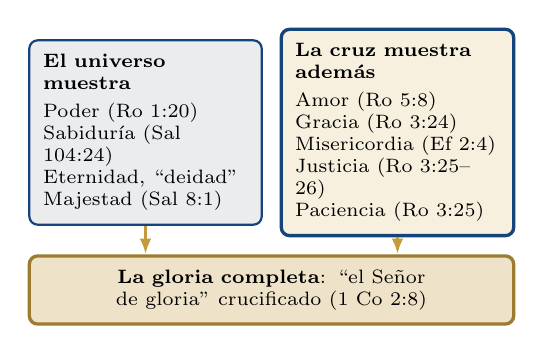
\begin{tikzpicture}[font=\tiny]
 \node[caja,text width=2.6cm,align=left,fill=gris!12] (u) at (0,0) {\textbf{El universo muestra}\\[2pt] Poder (Ro 1:20)\\ Sabiduría (Sal 104:24)\\ Eternidad, ``deidad''\\ Majestad (Sal 8:1)};
 \node[caja,text width=2.6cm,align=left,line width=1.2pt] (c) at (3.2,0) {\textbf{La cruz muestra además}\\[2pt] Amor (Ro 5:8)\\ Gracia (Ro 3:24)\\ Misericordia (Ef 2:4)\\ Justicia (Ro 3:25--26)\\ Paciencia (Ro 3:25)};
 \node[caja,text width=5.8cm,align=center,fill=dorado!30,draw=dorado!80!black,line width=1.2pt] (g) at (1.6,-2.0) {\textbf{La gloria completa}: ``el Señor de gloria'' crucificado (1 Co 2:8)};
 \draw[-{Latex[length=2mm]},dorado,line width=1.2pt] (u.south)--(u.south |- g.north);
 \draw[-{Latex[length=2mm]},dorado,line width=1.2pt] (c.south)--(c.south |- g.north);
\end{tikzpicture}
\end{column}
\end{columns}\par\smallskip
\scriptsize Tu material: ``el universo no refleja aquellos atributos como el amor, la gracia, la misericordia y la justicia\ldots{} Pero su Hijo en la cruz termina revelando\ldots{} la revelación de la gloria''.\ \precision{la creación muestra bondad general (Sal 145:9; Mt 5:45); no muestra el amor que perdona al culpable.}
\end{frame}

\begin{frame}{Destituidos de la gloria}
\begin{columns}[c,onlytextwidth]
\begin{column}{0.56\textwidth}
\begin{cita}Por cuanto todos pecaron, y están destituidos de la gloria de Dios, siendo justificados gratuitamente por su gracia, mediante la redención que es en Cristo Jesús, a quien Dios puso como propiciación por medio de la fe en su sangre, para manifestar su justicia, a causa de haber pasado por alto, en su paciencia, los pecados pasados\ldots\fuente{(Ro 3:23--25)}\end{cita}
\end{column}
\begin{column}{0.42\textwidth}\small
\begin{itemize}
\item \grc{ὑστεροῦνται}: ``quedarse corto'', presente: \destacar{siguen careciendo}.
\item En cuatro versos: gracia, justicia, paciencia, propiciación.
\item \grc{ἱλαστήριον}: el propiciatorio, donde la gloria se posaba (Lv 16:2).
\item Ro 5:2: ``nos gloriamos en la esperanza de la gloria de Dios''.
\end{itemize}
\end{column}
\end{columns}
\end{frame}

\begin{frame}{Las riquezas de su gloria}
\begin{cita}¿Y qué, si Dios, queriendo mostrar su ira y hacer notorio su poder, soportó con mucha paciencia los vasos de ira preparados para destrucción, y para hacer notorias las riquezas de su gloria, las mostró para con los vasos de misericordia que él preparó de antemano para gloria\ldots?\fuente{(Ro 9:22--23)}\end{cita}
\centering
\begin{tikzpicture}[font=\scriptsize]
 \foreach \x/\t [count=\k] in {0/Ira,2.2/Poder,4.4/Paciencia,6.6/Misericordia,8.8/Soberanía}{\node[caja,minimum width=1.9cm,align=center] (a\k) at (\x,0) {\t};}
 \node[caja,fill=dorado!30,draw=dorado!80!black,line width=1.2pt,text width=6cm,align=center] (g) at (4.4,-1.5) {``las riquezas de su gloria'' (\grc{τὸν πλοῦτον τῆς δόξης})};
 \foreach \k in {1,...,5}{\draw[-{Latex[length=2mm]},dorado,line width=1pt] (a\k.south)--(g);}
\end{tikzpicture}\par\smallskip
\scriptsize\RaggedRight Cinco atributos al servicio de un fin: la gloria. Ro 9:15 = Éx 33:19; Ro 9:17 = Éx 9:16. \precision{frase muy debatida (Moo, 1996); aquí solo se usa lo que el texto dice con claridad.}
\end{frame}

\begin{frame}{``Gloríese en el Señor''}
\scriptsize\renewcommand{\arraystretch}{1.2}
\begin{tabular}{@{}>{\RaggedRight\arraybackslash}p{3.5cm}>{\RaggedRight\arraybackslash}p{3.9cm}>{\RaggedRight\arraybackslash}p{4.0cm}@{}}
\toprule
\textbf{Jeremías 9:23--24} & \textbf{1 Corintios 1:26--31} & \textbf{Comentario} \\ \midrule
``el sabio en su sabiduría'' & ``no\ldots{} muchos sabios'' & la gloria intelectual \\
``el valiente'' & ``ni muchos poderosos'' & la gloria de la fuerza \\
``el rico'' & ``ni muchos nobles'' & la gloria social \\
``en entenderme y conocerme'' & ``Cristo\ldots{} hecho por Dios sabiduría'' & conocer a Dios es conocer a Cristo \\
``misericordia, juicio y justicia'' & ``justificación, santificación y redención'' & los atributos, dados en Cristo \\
\grc{ἐν τούτῳ καυχάσθω ὁ καυχώμενος} & \grc{ὁ καυχώμενος ἐν κυρίῳ καυχάσθω} & cita abreviada (1 Co 1:31) \\
\bottomrule
\end{tabular}\par\medskip
\small El verso de toda la obra, en Pablo: el ``Señor'' (\grc{κύριος}) que traduce el tetragrama es ahora Jesús. 1 Co 2:8: ``nunca habrían crucificado al \destacar{Señor de gloria}'' (Sal 24).\par
\precision{lectura de la mayoría de los comentaristas (Fee, 1987; Hays, 1989).}
\end{frame}

% ------------------------------------------------------------------
\section{De gloria en gloria}

\begin{frame}{Dos ministerios}
\begin{columns}[c,onlytextwidth]
\begin{column}{0.44\textwidth}
\begin{cita}Y si el ministerio de muerte grabado con letras en piedras fue con gloria, tanto que los hijos de Israel no pudieron fijar la vista en el rostro de Moisés a causa de la gloria de su rostro, la cual había de perecer, ¿cómo no será más bien con gloria el ministerio del espíritu?\fuente{(2 Co 3:7--8)}\end{cita}
\end{column}
\begin{column}{0.54\textwidth}
\scriptsize\renewcommand{\arraystretch}{1.12}
\begin{tabular}{@{}>{\RaggedRight\arraybackslash}p{0.8cm}>{\RaggedRight\arraybackslash}p{2.6cm}>{\RaggedRight\arraybackslash}p{2.8cm}@{}}
\toprule
& \textbf{Moisés (``con gloria'')} & \textbf{Espíritu (``mucho más'')} \\ \midrule
3:6 & ``la letra mata'' & ``el espíritu vivifica'' \\
3:7--8 & ministerio de muerte & ministerio del espíritu \\
3:9 & de condenación & de justificación \\
3:10 & ``lo que fue glorioso'' & ``la gloria más eminente'' \\
3:11 & ``lo que perece'' & ``lo que permanece'' \\
3:13, 18 & velo sobre el rostro & ``a cara descubierta'' \\
\bottomrule
\end{tabular}\par\smallskip
\emph{Qal vajómer} (de lo menor a lo mayor), la primera regla atribuida a Hilel. \destacar{No desprecia la Torá}: afirma que tuvo gloria.
\end{column}
\end{columns}
\end{frame}

\begin{frame}{El velo se quita}
\scriptsize\renewcommand{\arraystretch}{1.25}
\begin{tabular}{@{}>{\RaggedRight\arraybackslash}p{5.7cm}>{\RaggedRight\arraybackslash}p{5.7cm}@{}}
\toprule
\textbf{Éx 34:34 (LXX)} & \textbf{2 Co 3:16} \\ \midrule
\grc{ἡνίκα δ᾿ ἂν εἰσεπορεύετο Μωυσῆς ἔναντι κυρίου\ldots{} περιῃρεῖτο τὸ κάλυμμα} & \grc{ἡνίκα δὲ ἐὰν ἐπιστρέψῃ πρὸς κύριον, περιαιρεῖται τὸ κάλυμμα} \\
``Cuando Moisés entraba delante del Señor\ldots{} se quitaba el velo'' & ``Pero cuando se conviertan al Señor, el velo se quitará'' \\
\bottomrule
\end{tabular}\par\medskip
\small
\begin{itemize}
\item Lo que Moisés hacía al entrar a la presencia de Dios, lo hace \destacar{todo el que se vuelve al Señor}.
\item ``Porque el Señor es el Espíritu; y donde está el Espíritu del Señor, allí hay libertad'' (v. 17).
\end{itemize}
\precision{2 Co 3:7--18 como comentario (\emph{midrash}) de Éx 34:29--35 (Hafemann, 1995; Hays, 1989). Quién es el ``Señor'' del v. 17 se discute.}
\end{frame}

\begin{frame}{De gloria en gloria}
\fotolado{panel_2corintios3.jpg}{Elaboración propia: 2 Co 3:18b en escritura uncial (texto NA28).}
\begin{columns}[c,onlytextwidth]
\begin{column}{0.57\textwidth}
\begin{cita}Por tanto, nosotros todos, mirando a cara descubierta como en un espejo la gloria del Señor, somos transformados de gloria en gloria en la misma imagen, como por el Espíritu del Señor.\fuente{(2 Co 3:18)}\end{cita}
\scriptsize
\grc{ἀνακεκαλυμμένῳ προσώπῳ}: perfecto, el velo fue quitado y sigue quitado.\par
\grc{κατοπτριζόμενοι}: ``mirando como en un espejo'' o ``reflejando'' (Harris, 2005; Thrall, 1994).\par
\grc{μεταμορφούμεθα}: presente y pasivo: \destacar{proceso continuo, obra de otro}. El verbo de la transfiguración (Mt 17:2) y de Ro 12:2.\par
\grc{ἀπὸ δόξης εἰς δόξαν}: un grado de gloria a otro; cf. ``de poder en poder'' (\heb{מֵחַיִל אֶל־חָיִל}, Sal 84:7).
\end{column}
\begin{column}{0.41\textwidth}\end{column}
\end{columns}
\end{frame}

\begin{frame}{La gloria que crece}
\centering
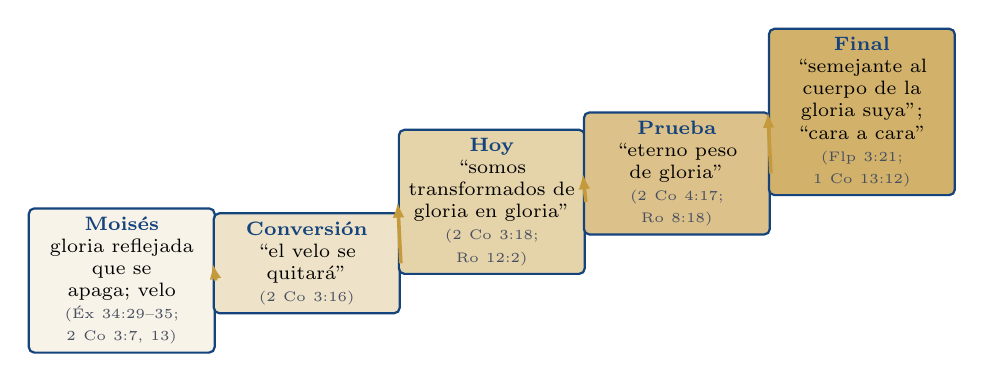
\begin{tikzpicture}[font=\scriptsize]
 \foreach \i/\t/\d/\r in {0/{Moisés}/{gloria reflejada que se apaga; velo}/{Éx 34:29--35; 2 Co 3:7, 13},1/{Conversión}/{``el velo se quitará''}/{2 Co 3:16},2/{Hoy}/{``somos transformados de gloria en gloria''}/{2 Co 3:18; Ro 12:2},3/{Prueba}/{``eterno peso de gloria''}/{2 Co 4:17; Ro 8:18},4/{Final}/{``semejante al cuerpo de la gloria suya''; ``cara a cara''}/{Flp 3:21; 1 Co 13:12}}{
   \pgfmathsetmacro{\x}{\i*2.35} \pgfmathsetmacro{\y}{\i*0.5} \pgfmathsetmacro{\c}{12+\i*16}
   \node[draw=azul,line width=0.8pt,fill=dorado!\c,rounded corners=2pt,text width=2.15cm,align=center,inner sep=3pt,anchor=south] (s\i) at (\x,\y) {\textbf{\textcolor{azul}{\t}}\\ \d\\ {\tiny\color{gris}(\r)}};}
 \foreach \i/\j in {0/1,1/2,2/3,3/4}{\draw[-{Latex[length=2mm]},dorado,line width=1.3pt] (s\i.east)--(s\j.west);}
\end{tikzpicture}\par\medskip
\begin{columns}[t,onlytextwidth]
\begin{column}{0.48\textwidth}\small Sal 115:8 invertido: el que mira ídolos se hace como ellos; \destacar{el que mira la gloria del Señor se hace como Él}.\end{column}
\begin{column}{0.48\textwidth}\small Col 3:10: el nuevo hombre ``conforme a la imagen del que lo creó se va renovando hasta el conocimiento pleno''.\end{column}
\end{columns}
\end{frame}

\begin{frame}{En la faz de Jesucristo}
\begin{cita}Porque Dios, que mandó que de las tinieblas resplandeciese la luz, es el que resplandeció en nuestros corazones, para iluminación del conocimiento de la gloria de Dios en la faz de Jesucristo.\fuente{(2 Co 4:6)}\end{cita}
\scriptsize\renewcommand{\arraystretch}{1.2}
\begin{tabular}{@{}>{\RaggedRight\arraybackslash}p{4.0cm}>{\RaggedRight\arraybackslash}p{3.4cm}>{\RaggedRight\arraybackslash}p{4.0cm}@{}}
\toprule
\textbf{Frase} & \textbf{Eco} & \textbf{Sentido} \\ \midrule
``de las tinieblas resplandeciese la luz'' & Gn 1:3; Is 9:2 & cada conversión es una nueva creación \\
``el conocimiento de la gloria'' & Hab 2:14 (LXX \grc{γνῶναι τὴν δόξαν}) & ensanchar el conocimiento de Dios \\
``en la faz'' (\grc{ἐν προσώπῳ}) & Éx 33:20 & el rostro negado a Moisés, mostrado en Cristo \\
\bottomrule
\end{tabular}\par\medskip
\small Damasco: ``no veía a causa de la gloria de la luz'' (Hch 22:11).
\end{frame}

\begin{frame}{Un eterno peso de gloria}
\begin{columns}[c,onlytextwidth]
\begin{column}{0.52\textwidth}
\begin{cita}Porque esta leve tribulación momentánea produce en nosotros un cada vez más excelente y eterno peso de gloria; no mirando nosotros las cosas que se ven, sino las que no se ven.\fuente{(2 Co 4:17--18)}\end{cita}
\end{column}
\begin{column}{0.46\textwidth}
\centering
\begin{tikzpicture}[font=\scriptsize]
 \draw[line width=2pt,azuloscuro] (-2.3,0.3)--(2.3,-0.5);
 \fill[azuloscuro] (0,-0.1)--(-0.3,-0.9)--(0.3,-0.9)--cycle;
 \node[caja,text width=1.7cm,align=center,fill=gris!12] at (-2.0,0.95) {``leve tribulación''\\ \grc{ἐλαφρόν}};
 \node[caja,text width=1.9cm,align=center,fill=dorado!35,draw=dorado!80!black] at (2.0,0.15) {``eterno \textbf{peso} de gloria''\\ \grc{βάρος δόξης}};
\end{tikzpicture}\par\smallskip
\small Un judío que piensa en hebreo (\emph{kavod} = peso) y escribe en griego: la gloria \destacar{pesa}.
\end{column}
\end{columns}\par\smallskip
\precision{el juego con \emph{kavod} es propuesta de los comentarios (Harris, 2005); el contraste ``leve / peso'' sí está en el griego.}
\end{frame}

% ------------------------------------------------------------------
\section{Colosenses}

\begin{frame}{Toda la plenitud}
\fotolado{panel_colosenses2.jpg}{Elaboración propia: Col 2:9 en escritura uncial (texto NA28).}
\begin{columns}[c,onlytextwidth]
\begin{column}{0.57\textwidth}
\begin{cita}El es la imagen del Dios invisible, el primogénito de toda creación\ldots{} por cuanto agradó al Padre que en él habitase toda plenitud.\fuente{(Col 1:15, 19)}\end{cita}
\begin{cita}Porque en él habita corporalmente toda la plenitud de la Deidad, y vosotros estáis completos en él.\fuente{(Col 2:9--10)}\end{cita}
\scriptsize Colosas buscaba plenitud en ``filosofías'', ángeles y rituales (2:8, 16--18). Pablo: \destacar{toda la plenitud ya está en Cristo}.
\end{column}
\begin{column}{0.41\textwidth}\end{column}
\end{columns}
\end{frame}

\begin{frame}{Filología de la plenitud}
\scriptsize\renewcommand{\arraystretch}{1.18}
\begin{tabular}{@{}>{\RaggedRight\arraybackslash}p{3.8cm}>{\RaggedRight\arraybackslash}p{7.8cm}@{}}
\toprule
\textbf{Griego} & \textbf{Sentido} \\ \midrule
\grc{εἰκὼν τοῦ θεοῦ τοῦ ἀοράτου} & ``imagen del Dios invisible'' (1:15): lo que no se ve de Dios se ve en el Hijo (Éx 33:20; Jn 1:18). \\
\grc{εὐδόκησεν\ldots{} κατοικῆσαι} & ``agradó\ldots{} que habitase'' (1:19). Posible eco del Sal 67:17 LXX [68:16]: ``el monte que quiso Dios para su morada''. \\
\grc{πλήρωμα} & ``plenitud'': la totalidad de lo que Dios es; recuerda el ``llenar'' de la gloria (\heb{מָלֵא}, Éx 40:34). \\
\grc{θεότητος} & ``de la Deidad'' (2:9): el ser mismo de Dios, no solo su cualidad (\grc{θειότης}, Ro 1:20). \\
\grc{σωματικῶς} & ``corporalmente'': habita ahora, en el Cristo resucitado. \\
\grc{πεπληρωμένοι} & ``completos'' (2:10): ``habéis sido \destacar{llenados}'': plenitud en Él, llenos en Él. \\
\bottomrule
\end{tabular}\par\medskip
\precision{autoría de Colosenses discutida (Moo, 2008); la idea tiene respaldo en cartas indiscutidas (2 Co 4:6; Flp 2:6; 1 Co 1:24). El eco del Sal 68 es propuesta.}
\end{frame}

\begin{frame}{Cuatro afirmaciones}
\centering
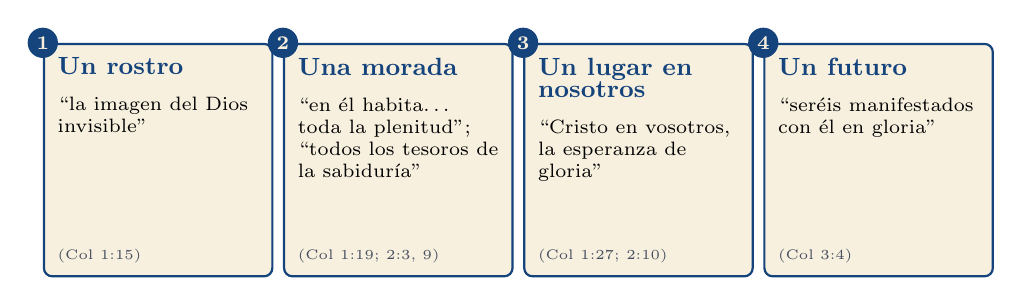
\begin{tikzpicture}
 \foreach \x/\n/\t/\d/\r in {0/1/{Un rostro}/{``la imagen del Dios invisible''}/{Col 1:15},
   3.05/2/{Una morada}/{``en él habita\ldots{} toda la plenitud''; ``todos los tesoros de la sabiduría''}/{Col 1:19; 2:3, 9},
   6.1/3/{Un lugar en nosotros}/{``Cristo en vosotros, la esperanza de gloria''}/{Col 1:27; 2:10},
   9.15/4/{Un futuro}/{``seréis manifestados con él en gloria''}/{Col 3:4}}{
  \node[caja,anchor=north] (b\n) at (\x,0) {\parbox[t][2.6cm][t]{2.55cm}{\RaggedRight
    {\small\textbf{\textcolor{azul}{\t}}}\\[5pt]\scriptsize \d\par\vfill{\tiny\color{gris}(\r)}}};
  \node[circle,fill=azul,text=papiro,font=\scriptsize\bfseries,inner sep=1.6pt] at (b\n.north west) {\n};}
\end{tikzpicture}\par\medskip
\small\RaggedRight Col 1:11: ``fortalecidos con todo poder, \destacar{conforme a la potencia de su gloria}, para toda paciencia y longanimidad''. La gloria también sostiene.
\end{frame}

\begin{frame}{Todos convergen en Cristo}
\centering
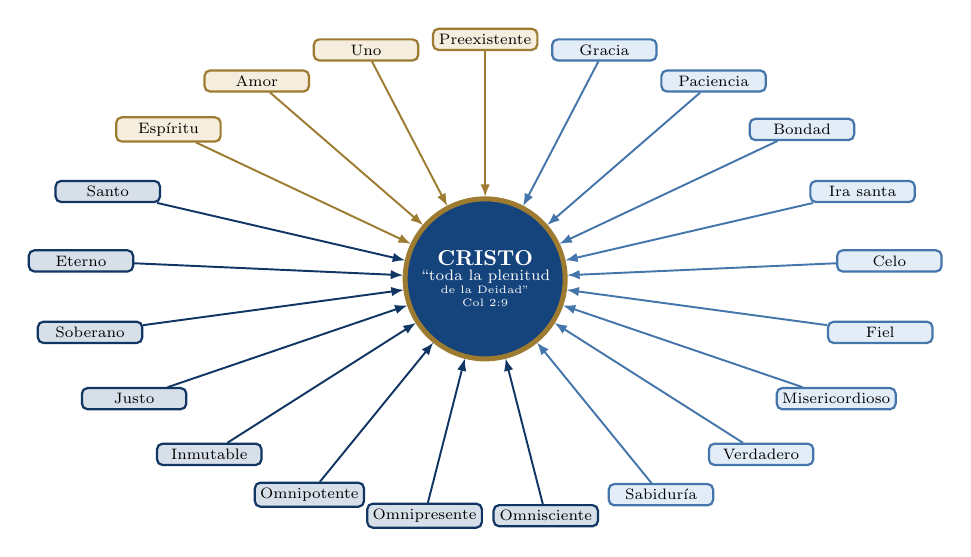
\begin{tikzpicture}[font=\tiny,scale=0.78,transform shape]
 \node[circle,draw=dorado!80!black,line width=1.8pt,fill=azul,text=white,minimum size=2.5cm,align=center] (c) at (0,0) {\normalsize\textbf{CRISTO}\\[1pt] \scriptsize ``toda la plenitud\\ de la Deidad''\\ Col 2:9};
 \foreach \a/\t/\col [count=\k] in {90/Preexistente/dorado,107.1/Uno/dorado,124.3/Amor/dorado,141.4/Espíritu/dorado,158.6/Santo/azul,175.7/Eterno/azul,192.9/Soberano/azul,210/Justo/azul,227.1/Inmutable/azul,244.3/Omnipotente/azul,261.4/Omnipresente/azul,278.6/Omnisciente/azul,295.7/Sabiduría/celeste,312.9/Verdadero/celeste,330/Misericordioso/celeste,347.1/Fiel/celeste,4.3/Celo/celeste,21.4/Ira santa/celeste,38.6/Bondad/celeste,55.7/Paciencia/celeste,72.9/Gracia/celeste}{
   \node[draw=\col!80!black,line width=0.8pt,fill=\col!18,fill opacity=0.95,text opacity=1,rounded corners=2pt,inner sep=2.5pt,minimum width=1.7cm,font=\scriptsize] (n\k) at ({6.6*cos(\a)},{3.9*sin(\a)}) {\t};
   \draw[\col!80!black,line width=0.7pt,-{Latex[length=1.6mm]}] (n\k)--(c);}
\end{tikzpicture}\par\smallskip
{\fontsize{5}{6}\selectfont\color{gris}\textit{Nota.} Elaboración propia: los veintiún atributos de la serie convergen en Cristo (Col 1:19; 2:9). Dorado: Ser; azul: Identidad; celeste: Relación.\par}
\end{frame}

\begin{frame}{Los atributos en Cristo (1)}
\scriptsize\renewcommand{\arraystretch}{1.1}
\begin{tabular}{@{}>{\RaggedRight\arraybackslash}p{2.2cm}>{\RaggedRight\arraybackslash}p{6.9cm}>{\RaggedRight\arraybackslash}p{2.6cm}@{}}
\toprule
\textbf{Atributo} & \textbf{En Cristo} & \textbf{Texto} \\ \midrule
\multicolumn{3}{@{}l}{\textcolor{azul}{\textbf{I. Ser}}} \\
Preexistente & ``como el Padre tiene vida en sí mismo, así también ha dado al Hijo el tener vida en sí mismo'' & Jn 5:26; Col 1:17 \\
Uno & ``un Señor, Jesucristo, por medio del cual son todas las cosas'' & 1 Co 8:6 (Dt 6:4) \\
Amor & ``el Hijo de Dios, el cual me amó y se entregó a sí mismo por mí'' & Gá 2:20 \\
Espíritu & ``el postrer Adán, espíritu vivificante'' & 1 Co 15:45 \\
\multicolumn{3}{@{}l}{\textcolor{azul}{\textbf{II. Identidad}}} \\
Santo & ``al que no conoció pecado'' & 2 Co 5:21; Hch 3:14 \\
Eterno & ``él es antes de todas las cosas'' & Col 1:17; Jn 8:58 \\
Soberano & ``todo fue creado por medio de él y para él'' & Col 1:16 \\
Justo & ``nos ha sido hecho por Dios\ldots{} justificación'' & 1 Co 1:30 \\
Inmutable & ``el mismo ayer, y hoy, y por los siglos'' & He 13:8 \\
Omnipotente & ``el poder con el cual puede también sujetar a sí mismo todas las cosas'' & Flp 3:21 \\
Omnipresente & ``la plenitud de Aquel que todo lo llena en todo'' & Ef 1:23 \\
Omnisciente & ``todos los tesoros de la sabiduría y del conocimiento'' & Col 2:3 \\
\bottomrule
\end{tabular}
\end{frame}

\begin{frame}{Los atributos en Cristo (2)}
\scriptsize\renewcommand{\arraystretch}{1.12}
\begin{tabular}{@{}>{\RaggedRight\arraybackslash}p{2.2cm}>{\RaggedRight\arraybackslash}p{6.9cm}>{\RaggedRight\arraybackslash}p{2.6cm}@{}}
\toprule
\textbf{Atributo} & \textbf{En Cristo} & \textbf{Texto} \\ \midrule
\multicolumn{3}{@{}l}{\textcolor{azul}{\textbf{III. Relación}}} \\
Sabiduría & ``Cristo poder de Dios, y sabiduría de Dios'' & 1 Co 1:24, 30 \\
Verdadero & ``la verdad que está en Jesús'' & Ef 4:21; Jn 14:6 \\
Misericordioso & ``Dios, que es rico en misericordia\ldots{} nos dio vida juntamente con Cristo'' & Ef 2:4--5 \\
Fiel & ``todas las promesas de Dios son en él Sí'' & 2 Co 1:20; 2 Ti 2:13 \\
Celo & ``El celo de tu casa me consume''; ``os celo con celo de Dios'' & Jn 2:17; 2 Co 11:2 \\
Ira santa & ``cuando se manifieste el Señor Jesús\ldots{} en llama de fuego'' & 2 Ts 1:7--8 \\
Bondad & ``se manifestó la bondad de Dios nuestro Salvador'' & Tit 3:4 \\
Paciencia & ``para que Jesucristo mostrase en mí\ldots{} toda su clemencia'' & 1 Ti 1:16 \\
Gracia & ``la gracia de nuestro Señor Jesucristo, que\ldots{} se hizo pobre'' & 2 Co 8:9 \\
\bottomrule
\end{tabular}\par\medskip
\precision{Juan, Hechos y Hebreos se usan donde Pablo no tiene un texto tan directo; Efesios, Colosenses, 2 Tesalonicenses y las Pastorales son de autoría discutida.}
\end{frame}

\begin{frame}{En la cruz se encontraron}
\scriptsize\renewcommand{\arraystretch}{1.16}
\begin{columns}[c,onlytextwidth]
\begin{column}{0.34\textwidth}\small
Sal 85:10: ``La misericordia y la verdad se encontraron; la justicia y la paz se besaron''.\par\medskip
En la cruz Dios es ``\destacar{el justo, y el que justifica}'' (Ro 3:26); ``haciendo la paz mediante la sangre de su cruz'' (Col 1:20). Ningún atributo anula a otro.
\end{column}
\begin{column}{0.64\textwidth}
\begin{tabular}{@{}>{\RaggedRight\arraybackslash}p{2.5cm}>{\RaggedRight\arraybackslash}p{3.3cm}>{\RaggedRight\arraybackslash}p{1.6cm}@{}}
\toprule
\textbf{Éx 34:6--7} & \textbf{En la cruz} & \textbf{Pablo} \\ \midrule
``misericordioso'' & ``rico en misericordia\ldots{} nos dio vida'' & Ef 2:4--5 \\
``piadoso'' & ``justificados gratuitamente por su gracia'' & Ro 3:24 \\
``tardo para la ira'' & ``en su paciencia'' & Ro 3:25 \\
``misericordia y verdad'' & ``para mostrar la verdad de Dios'' & Ro 15:8 \\
``perdona la iniquidad'' & ``el perdón de pecados'' & Col 1:14 \\
``de ningún modo tendrá por inocente'' & ``para manifestar su justicia'' & Ro 3:25--26 \\
\bottomrule
\end{tabular}
\end{column}
\end{columns}\par\smallskip
\precision{correspondencia propia: Pablo no cita Éx 34:6--7 en estos textos; sí cita Éx 33:19 en Ro 9:15.}
\end{frame}

\begin{frame}{Glorificados con Él}
\begin{columns}[c,onlytextwidth]
\begin{column}{0.50\textwidth}
\begin{cita}Y si hijos, también herederos; herederos de Dios y coherederos con Cristo, si es que padecemos juntamente con él, para que juntamente con él seamos glorificados.\fuente{(Ro 8:17)}\end{cita}
\begin{cita}Se siembra en deshonra, resucitará en gloria; se siembra en debilidad, resucitará en poder.\fuente{(1 Co 15:43)}\end{cita}
\end{column}
\begin{column}{0.48\textwidth}\small
\begin{itemize}
\item ``a los que justificó, a éstos también glorificó'' (\grc{ἐδόξασεν}, Ro 8:30): aoristo, \destacar{tan seguro como la justificación}.
\item ``destituidos de la gloria'' (Ro 3:23) $\rightarrow$ ``la esperanza de la gloria'' (Ro 5:2). Entre los dos, la cruz.
\item Pink (2020, p. 101): ``Hay una gran diferencia entre que los santos sean glorificados y que sean hechos divinos''.
\end{itemize}
\end{column}
\end{columns}
\end{frame}

% ------------------------------------------------------------------
\section{Vivirlo}

\begin{frame}{Solo a Dios la gloria}
\begin{columns}[t,onlytextwidth]
\begin{column}{0.49\textwidth}\small
\begin{enumerate}
\item \destacar{Renunciar a la gloria propia}: ``No a nosotros'' (Sal 115:1); ``ni buscamos gloria de los hombres'' (1 Ts 2:6).
\item \destacar{Gloriarse en conocer a Dios}: ``en entenderme y conocerme'' (Jer 9:24; 1 Co 1:31).
\item \destacar{Ensanchar la opinión} que otros tienen de Dios: ``glorifiquen a vuestro Padre'' (Mt 5:16; Hab 2:14).
\end{enumerate}
\end{column}
\begin{column}{0.49\textwidth}\small
\begin{enumerate}\setcounter{enumi}{3}
\item \destacar{Hacerlo todo para su gloria}: ``si, pues, coméis o bebéis'' (1 Co 10:31; Col 3:17).
\item \destacar{Ser iglesia} que muestra la ``multiforme sabiduría'' (\grc{πολυποίκιλος}) (Ef 3:10, 21).
\item \destacar{Contemplar y esperar}: ``de gloria en gloria'' (2 Co 3:18); ``eterno peso de gloria'' (2 Co 4:17).
\end{enumerate}
\end{column}
\end{columns}\par\medskip
\small\RaggedRight La advertencia de Elí: Israel quiso \destacar{la presencia sin la gloria}, el arca sin obediencia. La gloria de Dios no se usa: se honra (1 S 2:30).
\end{frame}

\begin{frame}{Para gloria de Dios}
\begin{columns}[c,onlytextwidth]
\begin{column}{0.50\textwidth}
\begin{cita}Si, pues, coméis o bebéis, o hacéis otra cosa, hacedlo todo para la gloria de Dios.\fuente{(1 Co 10:31)}\end{cita}
\begin{cita}para que la multiforme sabiduría de Dios sea ahora dada a conocer por medio de la iglesia a los principados y potestades en los lugares celestiales.\fuente{(Ef 3:10)}\end{cita}
\end{column}
\begin{column}{0.48\textwidth}\small
\begin{itemize}
\item Tu material: ``Dios hace todo para su propia gloria y la iglesia como institución no sería la excepción'' (Is 43:7; Ro 11:36).
\item ``La iglesia es un \destacar{instrumento de enseñanza y de glorificación} en las manos de Dios''.
\item Una iglesia reconciliada es la exposición pública de los atributos de Dios.
\end{itemize}
\end{column}
\end{columns}
\end{frame}

\begin{frame}{Para la reflexión}
\small
\begin{enumerate}\setlength{\itemsep}{6pt}
\item ¿En qué estoy poniendo el \destacar{peso} de mi vida: sabiduría, fuerza, riqueza, fama (Jer 9:23)?
\item ¿Busco ``la gloria de los hombres'' más que ``la gloria de Dios'' (Jn 12:43)?
\item ¿Mi manera de vivir \destacar{ensancha o achica} la opinión que otros tienen de Dios?
\item ¿Qué estoy contemplando? Uno se parece a lo que mira (Sal 115:8; 2 Co 3:18).
\item ¿Quiero la presencia de Dios como Israel en Afec, para que me salve, sin obedecerle (1 S 4:3)?
\item ¿Puedo mirar mi ``leve tribulación'' a la luz del ``eterno peso de gloria'' (2 Co 4:17)?
\end{enumerate}
\end{frame}

% ------------------------------------------------------------------
\section{Síntesis}

\begin{frame}{La gloria de Dios}
\begin{tcolorbox}[enhanced,colback=papiro,colframe=azul,boxrule=1pt,arc=3pt,title={Síntesis},fonttitle=\bfseries\small,colbacktitle=azul,coltitle=papiro,fontupper=\small]
La gloria de Dios es \destacar{la comunión perfecta de todos sus atributos}: el \emph{kavod}, el peso infinito de lo que Dios es (Éx 33:18--34:7). Se manifiesta en la creación (Sal 19:1; Ro 1:20), en la historia de Israel (Éx 40:34; 2 Cr 7:1) y, en plenitud, en Jesucristo, en quien ``habita corporalmente toda la plenitud de la Deidad'' (Col 2:9) y en cuyo rostro brilla ``el conocimiento de la gloria de Dios'' (2 Co 4:6). No se comparte con los ídolos (Is 42:8), pero se comunica a los que están en Cristo, transformados ``de gloria en gloria'' (2 Co 3:18). Al ser humano le corresponde reconocerla: ``No a nosotros\ldots{} sino a tu nombre da gloria'' (Sal 115:1).
\end{tcolorbox}
\end{frame}

\begin{frame}{Gloria de Dios: su esencia infinita}
\imagen[0.80]{gloria_esquema.jpg}{Esquema del autor de la serie: los atributos del Ser, de la Identidad y de la Relación, sincronizados por la Sabiduría.}
\end{frame}

\begin{frame}{Cuatro miradas}
\scriptsize\renewcommand{\arraystretch}{1.2}
\begin{tabular}{@{}>{\RaggedRight\arraybackslash}p{1.8cm}>{\RaggedRight\arraybackslash}p{9.8cm}@{}}
\toprule
\textbf{Mirada} & \textbf{Aporte a la gloria} \\ \midrule
Hebrea & \emph{kavod}, ``peso''; la gloria que desciende, reposa, llena, habla y se va; Elí ``pesado'' e Icabod; el Nombre como gloria proclamada (Éx 34:6--7); la nube que baja cuando se cantan los atributos (2 Cr 5:13--14). \\
Judía & La Shejiná que acompaña al pueblo al exilio (\emph{Meguilá} 29a); el segundo templo sin Shejiná (\emph{Yomá} 21b); todo creado para su gloria (\emph{Avot} 6:11); la \emph{Qedushá}; Maimónides. \\
Pink & La gloria esencial no aumenta ni disminuye; crece su reconocimiento; ``el nombre es la colección de sus Atributos''. \\
Paulina & La creación y la cruz (Ro 1; 3); ``gloríese en el Señor'' (1 Co 1:31); ``de gloria en gloria'' (2 Co 3:18); ``eterno peso de gloria''; toda la plenitud en Cristo (Col 1:19; 2:9). \\
\bottomrule
\end{tabular}\par\bigskip
\begin{cita}Porque de él, y por él, y para él, son todas las cosas. A él sea la gloria por los siglos. Amén.\fuente{(Ro 11:36)}\end{cita}
\end{frame}


\begin{frame}{Glosario}
\scriptsize
\begin{columns}[t,onlytextwidth]
\begin{column}{0.49\textwidth}
\begin{description}\setlength{\itemsep}{1pt}
\item[\emph{Aspaqlaria}] (\heb{אַסְפַּקְלַרְיָא}) espejo, vidrio (\emph{Yevamot} 49b).
\item[\emph{Doxa}] (\grc{δόξα}) opinión; en la LXX y el NT, gloria, resplandor.
\item[\emph{Doxazō}] (\grc{δοξάζω}) glorificar (Jn 12:28; Ro 8:30).
\item[\emph{Eskēnōsen}] (\grc{ἐσκήνωσεν}) ``puso su tienda'' (Jn 1:14).
\item[\emph{Hashem hanijbad}] (\heb{הַשֵּׁם הַנִּכְבָּד}) ``el nombre glorioso'' (Dt 28:58).
\item[\emph{Hithalel}] (\heb{הִתְהַלֵּל}) gloriarse (Jer 9:23--24).
\item[\emph{Icabod}] (\heb{אִי־כָבוֹד}) ``¿dónde está la gloria?'' (1 S 4:21).
\item[\emph{Kaved}] (\heb{כָּבֵד}) pesado; \emph{kibbed}, honrar.
\item[\emph{Kavod}] (\heb{כָּבוֹד}) peso, honra, gloria.
\end{description}
\end{column}
\begin{column}{0.49\textwidth}
\begin{description}\setlength{\itemsep}{1pt}
\item[\emph{Metamorphoō}] (\grc{μεταμορφόω}) transformar (2 Co 3:18).
\item[\emph{Mishkán}] (\heb{מִשְׁכָּן}) morada, tabernáculo.
\item[\emph{Plērōma}] (\grc{πλήρωμα}) plenitud (Col 1:19; 2:9).
\item[\emph{Qal vajómer}] argumento de lo menor a lo mayor (2 Co 3:7--11).
\item[\emph{Qedushá}] (\heb{קְדֻשָּׁה}) oración que une Is 6:3 y Ez 3:12.
\item[\emph{Shejiná}] (\heb{שְׁכִינָה}) la presencia que habita.
\item[\emph{Theotēs}] (\grc{θεότης}) Deidad (Col 2:9); \grc{θειότης}, cualidad divina (Ro 1:20).
\item[\emph{Yarad}] (\heb{יָרַד}) descender (Éx 33:9; 34:5).
\item[\emph{Yeqará}] (\heb{יְקָרָא}) honra; el \emph{kavod} en Ónkelos.
\end{description}
\end{column}
\end{columns}
\end{frame}

% ------------------------------------------------------------------
\section{Referencias}

\begin{frame}[allowframebreaks]{Referencias}
\tiny
\refapa{Alter, R. (1999). \emph{The David story: A translation with commentary of 1 and 2 Samuel}. W.~W. Norton.}
\refapa{Bauckham, R. (2008). \emph{Jesus and the God of Israel}. Eerdmans.}
\refapa{\emph{Bereshit Rabá} [12:6]. (s.f.). Sefaria. \url{https://www.sefaria.org}}
\refapa{Berkhof, L. (1938). \emph{Systematic theology}. Eerdmans.}
\refapa{Brown, F., Driver, S.~R., \& Briggs, C.~A. (1906). \emph{A Hebrew and English lexicon of the Old Testament}. Clarendon Press.}
\refapa{Carson, D.~A. (1991). \emph{The Gospel according to John}. Eerdmans.}
\refapa{Charnock, S. (1996). \emph{The existence and attributes of God}. Baker Books. (Obra original publicada en 1682)}
\refapa{Elliger, K., \& Rudolph, W. (Eds.). (1997). \emph{Biblia Hebraica Stuttgartensia} (5.ª ed.). Deutsche Bibelgesellschaft.}
\refapa{Fee, G.~D. (1987). \emph{The first epistle to the Corinthians}. Eerdmans.}
\refapa{García Martínez, F. (1992). \emph{Textos de Qumrán}. Trotta.}
\refapa{Hafemann, S.~J. (1995). \emph{Paul, Moses, and the history of Israel}. Mohr Siebeck.}
\refapa{Harris, M.~J. (2005). \emph{The second epistle to the Corinthians}. Eerdmans.}
\refapa{Hays, R.~B. (1989). \emph{Echoes of Scripture in the letters of Paul}. Yale University Press.}
\refapa{Koehler, L., \& Baumgartner, W. (2001). \emph{The Hebrew and Aramaic lexicon of the Old Testament}. Brill.}
\refapa{Maimónides. (1903). \emph{The guide for the perplexed} [I:54; I:64] (M. Friedländer, Trad.). Routledge.}
\refapa{\emph{Misná: Pirqé Avot} [6:11]. (s.f.). Sefaria. \url{https://www.sefaria.org}}
\refapa{Moo, D.~J. (1996). \emph{The epistle to the Romans}. Eerdmans.}
\refapa{Moo, D.~J. (2008). \emph{The letters to the Colossians and to Philemon}. Eerdmans.}
\refapa{Nestle, E., \& Aland, K. (Eds.). (2012). \emph{Novum Testamentum Graece} (28.ª ed.). Deutsche Bibelgesellschaft.}
\refapa{Pink, A.~W. (2020). \emph{Los atributos de Dios} (E. Rodríguez Cruz, Trad.). Chapel Library. (Obra original publicada en 1930)}
\refapa{Rahlfs, A., \& Hanhart, R. (Eds.). (2006). \emph{Septuaginta} (Ed. rev.). Deutsche Bibelgesellschaft.}
\refapa{\emph{Santa Biblia: Reina-Valera 1960}. (1960). Sociedades Bíblicas en América Latina.}
\refapa{\emph{Shemot Rabá} [3:6]. (s.f.). Sefaria. \url{https://www.sefaria.org}}
\refapa{Steinsaltz, A. (Ed.). (2017). \emph{Koren Talmud Bavli} [Meguilá 29a; Shabat 30a; Yevamot 49b; Yomá 21b]. Sefaria.}
\refapa{\emph{Targum Ónkelos} [Éx 25:8; 33:20--22; 40:34]. (s.f.). Sefaria. \url{https://www.sefaria.org}}
\refapa{Thrall, M.~E. (1994). \emph{The second epistle to the Corinthians} (Vol. 1). T\&T Clark.}
\refapa{Trench, R.~C. (1880). \emph{Synonyms of the New Testament} (9.ª ed.). Macmillan.}
\refapa{Vine, W.~E. (1999). \emph{Diccionario expositivo de palabras del Antiguo y del Nuevo Testamento exhaustivo}. Caribe.}
\end{frame}

\end{document}
